%%%%%%%%%%%%%%%%%%%%%%%%%%%%%%%%%%%%%%%%%%%%%%%%%%%
\begin{frame}
  \begin{center}
    {\Large Introduction to TensorFlow}
    
    (Mostly referring CS20si Stanford slides and explanation by Labhesh Patel and Goolge ML crash course)
  \end{center}
\end{frame}


%%%%%%%%%%%%%%%%%%%%%%%%%%%%%%%%%%%%%%%%%%%%%%%%%%%
\begin{frame}[fragile] \frametitle{TensorFlow is}
\begin{itemize}
\item Open source, Free library, with Python bindings, by Google Brain team
\item Other libraries are: Caffe (Berkeley), Torch (Facebook), Cntk (Microsoft),
\item Can deploy computation to one or more CPUs or GPUs in a desktop, server, or mobile device with a single API
\item Flexibility: from Raspberry Pi, Android, Windows, iOS, Linux to server farms
\item Has simplified wrappers like: Keras, TF Learnbut we will do raw tf
\end{itemize}
\end{frame}


%%%%%%%%%%%%%%%%%%%%%%%%%%%%%%%%%%%%%%%%%%%%%%%%%%%
\begin{frame}[fragile] \frametitle{Goals}
\begin{itemize}
\item Understand TF's computation graph approach
\item Learn how to build and structure models best suited for a deep learning project.
\item Model business cases

\end{itemize}
\end{frame}


%%%%%%%%%%%%%%%%%%%%%%%%%%%%%%%%%%%%%%%%%%%%%%%%%%%
\begin{frame}[fragile] \frametitle{Installation}
\begin{itemize}
\item Windows 7, 64 bit on Python 3
\item Test
\begin{lstlisting}
Import tensorflow as tf
\end{lstlisting}
\end{itemize}
\end{frame}

%%%%%%%%%%%%%%%%%%%%%%%%%%%%%%%%%%%%%%%%%%%%%%%%%%%
\begin{frame}[fragile] \frametitle{Hello World!}
Here is a "Hello World" TensorFlow program:
\begin{lstlisting}
import tensorflow as tf

c = tf.constant('Hello, world!')
with tf.Session() as sess:
    print(sess.run(c))
\end{lstlisting}
\end{frame}

%%%%%%%%%%%%%%%%%%%%%%%%%%%%%%%%%%%%%%%%%%%%%%%%%%%
\begin{frame}[fragile] \frametitle{Concepts}
Basic data structures:
\begin{itemize}
\item tensors
\item operations
\item graphs
\item sessions
\end{itemize}
We will build a simple TensorFlow program that creates a default graph, and a session that runs the graph
\end{frame}


%%%%%%%%%%%%%%%%%%%%%%%%%%%%%%%%%%%%%%%%%%%%%%%%%%%
\begin{frame}[fragile] \frametitle{Graph}
\begin{itemize}
\item Problem is model as a graph (a network of nodes).
\item Nodes can be values or operations.
\item Data (n-dimensional, called Tensors) flows through the graph
\item Hence the name, TensorFlow
\end{itemize}
\begin{center}
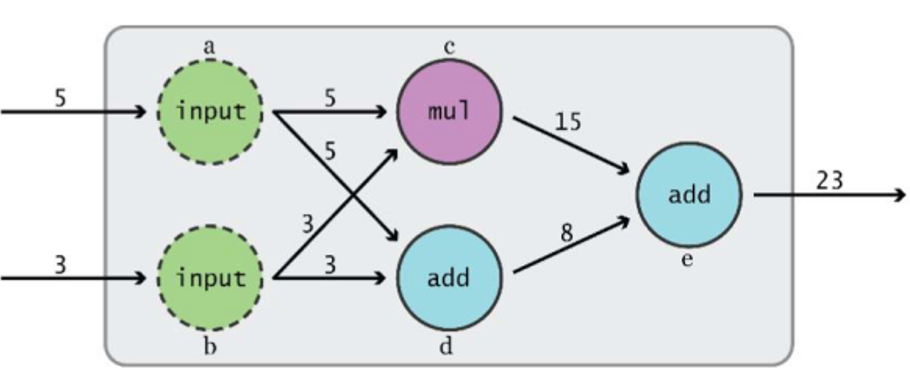
\includegraphics[width=0.8\linewidth,keepaspectratio]{tfgraph}
\end{center}
\end{frame}

%%%%%%%%%%%%%%%%%%%%%%%%%%%%%%%%%%%%%%%%%%%%%%%%%%%
\begin{frame}[fragile] \frametitle{Data flow Graph}
\begin{itemize}
\item TensorFlow separates definition of computations from their execution
\item Steps:
\begin{itemize}
\item assemble a graph
\item use a session to execute operations in the graph.
\end{itemize}
\item Why:
\begin{itemize}
\item Avoid continuous backend calls to C++ from Python program
\item Leverage parallelization and also GPU execution, wherever available
\end{itemize}
\end{itemize}
\end{frame}

%%%%%%%%%%%%%%%%%%%%%%%%%%%%%%%%%%%%%%%%%%%%%%%%%%%
\begin{frame}[fragile] \frametitle{What is a Tensor?}
\begin{itemize}
\item An n-dimensional vector
\begin{itemize}
\item 0-d tensor: scalar (number) : For example, "Howdy" or 5
\item 1-d tensor: vector:  For example, [2, 3, 5, 7, 11] or [5]
\item 2-d tensor: matrix: For example, [[3.1, 8.2, 5.9][4.3, -2.7, 6.5]]
\item and so on
\end{itemize}
\item Examples?: Stress at a point, Space-time event, etc
\end{itemize}
\end{frame}

%%%%%%%%%%%%%%%%%%%%%%%%%%%%%%%%%%%%%%%%%%%%%%%%%%%
\begin{frame}[fragile] \frametitle{What is an  Operation?}
\begin{itemize}
\item TensorFlow operations create, destroy, and manipulate tensors. 
\item Most of the lines of code in a typical TensorFlow program are operations.
\end{itemize}
\end{frame}

%%%%%%%%%%%%%%%%%%%%%%%%%%%%%%%%%%%%%%%%%%%%%%%%%%%
\begin{frame}[fragile] \frametitle{What is a Graph?}
\begin{itemize}
\item TensorFlow operations create, destroy, and manipulate tensors. 
\item Most of the lines of code in a typical TensorFlow program are operations.
\end{itemize}
\end{frame}

%%%%%%%%%%%%%%%%%%%%%%%%%%%%%%%%%%%%%%%%%%%%%%%%%%%
\begin{frame}[fragile] \frametitle{TensorFlow Graph}
\begin{itemize}
\item A TensorFlow graph (also known as a computational graph or a dataflow graph) is a graph data structure
\item A graph's nodes are operations; a graph's edges are tensors. 
\item Tensors flow through the graph, manipulated at each node by an operation. 
\item The output tensor of one operation often becomes the input tensor to a subsequent operation. 
\item TensorFlow implements a lazy execution model, meaning that nodes are only computed when needed, based on the needs of associated nodes.
\end{itemize}
\end{frame}


%%%%%%%%%%%%%%%%%%%%%%%%%%%%%%%%%%%%%%%%%%%%%%%%%%%
\begin{frame}[fragile] \frametitle{Tensors}
\begin{itemize}
\item Tensors can be stored in the graph as constants or variables. 
\item EVEN these are operations in TensorFlow
\item A constant is an operation that always returns the same tensor value. 
\item A variable is an operation that will return whichever tensor has been assigned to it.
\end{itemize}
\end{frame}

%%%%%%%%%%%%%%%%%%%%%%%%%%%%%%%%%%%%%%%%%%%%%%%%%%%
\begin{frame}[fragile] \frametitle{Tensors}
\begin{itemize}
\item To define a constant, use the tf.constant operator and pass in its value. For example:
\begin{lstlisting}
x = tf.constant(5.2)
\end{lstlisting}
\item Similarly, you can create a variable like this:
\begin{lstlisting}
y = tf.Variable([5])
\end{lstlisting}
\item Or you can create the variable first and then subsequently assign a value like this (note that you always have to specify a default value):
\begin{lstlisting}
y = tf.Variable([0])
  y = y.assign([5])
\end{lstlisting}
\end{itemize}
\end{frame}

%%%%%%%%%%%%%%%%%%%%%%%%%%%%%%%%%%%%%%%%%%%%%%%%%%%
\begin{frame}[fragile] \frametitle{Tensor Operations}
\begin{itemize}
\item Once you've defined some constants or variables, you can combine them with other operations like tf.add. 
\item When you evaluate the tf.add operation, it will call your tf.constant or tf.Variable operations to get their values and then return a new tensor with the sum of those values.
\end{itemize}
\end{frame}

%%%%%%%%%%%%%%%%%%%%%%%%%%%%%%%%%%%%%%%%%%%%%%%%%%%
\begin{frame}[fragile] \frametitle{Session}
Graphs must run within a TensorFlow session, which holds the state for the graph(s) it runs:
\begin{lstlisting}
with tf.Session() as sess:
  initialization = tf.global_variables_initializer()
  print(y.eval())
\end{lstlisting}
When working with tf.Variables, you must explicitly initialize them by calling tf.global\_variables\_initializer at the start of your session, as shown above.
\end{frame}

%%%%%%%%%%%%%%%%%%%%%%%%%%%%%%%%%%%%%%%%%%%%%%%%%%%
\begin{frame}[fragile] \frametitle{Summary}
TensorFlow programming is essentially a two-step process:
\begin{lstlisting}
Assemble constants, variables, and operations into a graph.
Evaluate those constants, variables and operations within a session.
\end{lstlisting}
\end{frame}


%%%%%%%%%%%%%%%%%%%%%%%%%%%%%%%%%%%%%%%%%%%%%%%%%%%
\begin{frame}[fragile] \frametitle{Small program}
Graphs must run within a TensorFlow session, which holds the state for the graph(s) it runs:
\begin{lstlisting}
import tensorflow as tf

# Create a graph.
g = tf.Graph()

# Establish the graph as the "default" graph.
with g.as_default():
  # Assemble a graph consisting of the following three operations:
  #   * Two tf.constant operations to create the operands.
  #   * One tf.add operation to add the two operands.
  x = tf.constant(8, name="x_const")
  y = tf.constant(5, name="y_const")
  my_sum = tf.add(x, y, name="x_y_sum")


  # Now create a session.
  # The session will run the default graph.
  with tf.Session() as sess:
    print(my_sum.eval()) # or print(sess.run(my_sum))
\end{lstlisting}
TensorFlow provides a default graph. However, we recommend explicitly creating your own Graph instead to facilitate tracking state (e.g., you may wish to work with a different Graph in each cell).
\end{frame}


%%%%%%%%%%%%%%%%%%%%%%%%%%%%%%%%%%%%%%%%%%%%%%%%%%%
\begin{frame}[fragile] \frametitle{Exercise: Introduce a Third Operand}
Revise the above code listing to add three integers, instead of two:
\begin{itemize}
\item Define a third scalar integer constant, z, and assign it a value of 4.
\item Add z to my\_sum to yield a new sum.
\item 
Hint: See the API docs for tf.add() (https://www.tensorflow.org/api\_docs/python/tf/add) for more details on its function signature.
\item 
Re-run the modified code block. Did the program generate the correct grand total?
\end{itemize}
\end{frame}


%%%%%%%%%%%%%%%%%%%%%%%%%%%%%%%%%%%%%%%%%%%%%%%%%%%
\begin{frame}[fragile] \frametitle{Example: How to get the value of $a$?}
\begin{itemize}
\item Create a session
\item Within the session, evaluate $a$ node
\begin{minipage}[t]{0.48\linewidth}
\begin{lstlisting}
import tensorflow as tf

a = tf.add(3, 5)
sess = tf.Session()
Print(sess.run(a))
sess.close()
>> 8
\end{lstlisting}
\end{minipage}
\hfill
\begin{minipage}[t]{0.48\linewidth}
\begin{lstlisting}
import tensorflow as tf

a = tf.add(3, 5)
with tf.Session() as sess:
    print(sess.run(a))
>> 8
\end{lstlisting}
\end{minipage}
\item A Session object encapsulates the environment in which Operation objects are executed, and Tensor objects are evaluate
\end{itemize}
\end{frame}

%%%%%%%%%%%%%%%%%%%%%%%%%%%%%%%%%%%%%%%%%%%%%%%%%%%
\begin{frame}[fragile] \frametitle{Vector Addition}
The following code creates and manipulates two vectors (1-D tensors), each having exactly six elements:
\begin{lstlisting}
import tensorflow as tf

with tf.Graph().as_default():
  # Create a six-element vector (1-D tensor).
  primes = tf.constant([2, 3, 5, 7, 11, 13], dtype=tf.int32)

  # Create another six-element vector. Each element in the vector will be
  # initialized to 1. The first argument is the shape of the tensor (more
  # on shapes below).
  ones = tf.ones([6], dtype=tf.int32)

  # Add the two vectors. The resulting tensor is a six-element vector.
  just_beyond_primes = tf.add(primes, ones)

  # Create a session to run the default graph.
  with tf.Session() as sess:
    print(just_beyond_primes.eval())
\end{lstlisting}
\end{frame}

%%%%%%%%%%%%%%%%%%%%%%%%%%%%%%%%%%%%%%%%%%%%%%%%%%%
\begin{frame}[fragile] \frametitle{Tensor Shapes}
\begin{itemize}
\item The shape of a tensor is expressed as list, with the ith element representing the size along dimension i. 
\item The length of the list then indicates the rank of the tensor (i.e., the number of dimensions).
\end{itemize}

\end{frame}

%%%%%%%%%%%%%%%%%%%%%%%%%%%%%%%%%%%%%%%%%%%%%%%%%%%
\begin{frame}[fragile] \frametitle{Tensor Shapes}

\begin{lstlisting}
import tensorflow as tf

with tf.Graph().as_default():
  # A scalar (0-D tensor).
  scalar = tf.zeros([])

  # A vector with 3 elements.
  vector = tf.zeros([3])

  # A matrix with 2 rows and 3 columns.
  matrix = tf.zeros([2, 3])

  with tf.Session() as sess:
    print('scalar has shape', scalar.get_shape(), 'and value:\n', scalar.eval())
    print('vector has shape', vector.get_shape(), 'and value:\n', vector.eval())
    print('matrix has shape', matrix.get_shape(), 'and value:\n', matrix.eval())
\end{lstlisting}

\end{frame}




%%%%%%%%%%%%%%%%%%%%%%%%%%%%%%%%%%%%%%%%%%%%%%%%%%%
\begin{frame}[fragile] \frametitle{Broadcasting}
\begin{itemize}
\item In mathematics, you can only perform element-wise operations (e.g. add and equals) on tensors of the same shape.
\item In TensorFlow, however, you may perform operations on tensors that would traditionally have been incompatible. 
\item TensorFlow supports broadcasting (a concept borrowed from numpy), where the smaller array in an element-wise operation is enlarged to have the same shape as the larger array. 
\item  When a tensor is broadcast, its entries are conceptually copied. (They are not actually copied for performance reasons. Broadcasting was invented as a performance optimization.)
\end{itemize}

\end{frame}



%%%%%%%%%%%%%%%%%%%%%%%%%%%%%%%%%%%%%%%%%%%%%%%%%%%
\begin{frame}[fragile] \frametitle{Broadcasting}
The following code performs the same tensor addition as before, but using broadcasting:
\begin{lstlisting}
import tensorflow as tf

with tf.Graph().as_default():
  # Create a six-element vector (1-D tensor).
  primes = tf.constant([2, 3, 5, 7, 11, 13], dtype=tf.int32)

  # Create a constant scalar with value 1.
  ones = tf.constant(1, dtype=tf.int32)

  # Add the two tensors. The resulting tensor is a six-element vector.
  just_beyond_primes = tf.add(primes, ones)

  with tf.Session() as sess:
    print(just_beyond_primes.eval())
\end{lstlisting}

\end{frame}

%%%%%%%%%%%%%%%%%%%%%%%%%%%%%%%%%%%%%%%%%%%%%%%%%%%
\begin{frame}[fragile] \frametitle{Matrix Multiplication}
\begin{itemize}
\item In linear algebra, when multiplying two matrices, the number of columns of the first matrix must equal the number of rows in the second matrix.
\item 
It is valid to multiply a 3x4 matrix by a 4x2 matrix. This will result in a 3x2 matrix.
\item  It is invalid to multiply a 4x2 matrix by a 3x4 matrix.
\end{itemize}
\end{frame}

%%%%%%%%%%%%%%%%%%%%%%%%%%%%%%%%%%%%%%%%%%%%%%%%%%%
\begin{frame}[fragile] \frametitle{Matrix Multiplication}
\begin{lstlisting}
import tensorflow as tf

with tf.Graph().as_default():
  # Create a matrix (2-d tensor) with 3 rows and 4 columns.
  x = tf.constant([[5, 2, 4, 3], [5, 1, 6, -2], [-1, 3, -1, -2]],
                  dtype=tf.int32)

  # Create a matrix with 4 rows and 2 columns.
  y = tf.constant([[2, 2], [3, 5], [4, 5], [1, 6]], dtype=tf.int32)

  # Multiply `x` by `y`. 
  # The resulting matrix will have 3 rows and 2 columns.
  matrix_multiply_result = tf.matmul(x, y)

  with tf.Session() as sess:
    print(matrix_multiply_result.eval())
\end{lstlisting}

\end{frame}

%%%%%%%%%%%%%%%%%%%%%%%%%%%%%%%%%%%%%%%%%%%%%%%%%%%
\begin{frame}[fragile] \frametitle{Tensor Reshaping}
\begin{itemize}
\item With tensor addition and matrix multiplication each imposing constraints on operands, TensorFlow programmers must frequently reshape tensors.
\item You can use the tf.reshape method to reshape a tensor. For example, you can reshape a 8x2 tensor into a 2x8 tensor or a 4x4 tensor:
\end{itemize}

\end{frame}


%%%%%%%%%%%%%%%%%%%%%%%%%%%%%%%%%%%%%%%%%%%%%%%%%%%
\begin{frame}[fragile] \frametitle{Tensor Reshaping}
\begin{lstlisting}
import tensorflow as tf

with tf.Graph().as_default():
  # Create an 8x2 matrix (2-D tensor).
  matrix = tf.constant([[1,2], [3,4], [5,6], [7,8],
                        [9,10], [11,12], [13, 14], [15,16]], dtype=tf.int32)

  # Reshape the 8x2 matrix into a 2x8 matrix.
  reshaped_2x8_matrix = tf.reshape(matrix, [2,8])
  
  # Reshape the 8x2 matrix into a 4x4 matrix
  reshaped_4x4_matrix = tf.reshape(matrix, [4,4])

  with tf.Session() as sess:
    print("Original matrix (8x2):")
    print(matrix.eval())
    print("Reshaped matrix (2x8):")
    print(reshaped_2x8_matrix.eval())
    print("Reshaped matrix (4x4):")
    print(reshaped_4x4_matrix.eval())
\end{lstlisting}

\end{frame}


%%%%%%%%%%%%%%%%%%%%%%%%%%%%%%%%%%%%%%%%%%%%%%%%%%%
\begin{frame}[fragile] \frametitle{Tensor Reshaping}
\begin{lstlisting}
import tensorflow as tf

with tf.Graph().as_default():
  # Create an 8x2 matrix (2-D tensor).
  matrix = tf.constant([[1,2], [3,4], [5,6], [7,8],
                        [9,10], [11,12], [13, 14], [15,16]], dtype=tf.int32)

  # Reshape the 8x2 matrix into a 3-D 2x2x4 tensor.
  reshaped_2x2x4_tensor = tf.reshape(matrix, [2,2,4])
  
  # Reshape the 8x2 matrix into a 1-D 16-element tensor.
  one_dimensional_vector = tf.reshape(matrix, [16])

  with tf.Session() as sess:
    print("Original matrix (8x2):")
    print(matrix.eval())
    print("Reshaped 3-D tensor (2x2x4):")
    print(reshaped_2x2x4_tensor.eval())
    print("1-D vector:")
    print(one_dimensional_vector.eval())
\end{lstlisting}

\end{frame}

%%%%%%%%%%%%%%%%%%%%%%%%%%%%%%%%%%%%%%%%%%%%%%%%%%%
\begin{frame}[fragile] \frametitle{Tensor Reshaping}
\begin{lstlisting}
import tensorflow as tf

with tf.Graph().as_default():
  # Create an 8x2 matrix (2-D tensor).
  matrix = tf.constant([[1,2], [3,4], [5,6], [7,8],
                        [9,10], [11,12], [13, 14], [15,16]], dtype=tf.int32)

  # Reshape the 8x2 matrix into a 3-D 2x2x4 tensor.
  reshaped_2x2x4_tensor = tf.reshape(matrix, [2,2,4])
  
  # Reshape the 8x2 matrix into a 1-D 16-element tensor.
  one_dimensional_vector = tf.reshape(matrix, [16])

  with tf.Session() as sess:
    print("Original matrix (8x2):")
    print(matrix.eval())
    print("Reshaped 3-D tensor (2x2x4):")
    print(reshaped_2x2x4_tensor.eval())
    print("1-D vector:")
    print(one_dimensional_vector.eval())
\end{lstlisting}

\end{frame}

%%%%%%%%%%%%%%%%%%%%%%%%%%%%%%%%%%%%%%%%%%%%%%%%%%%
\begin{frame}[fragile] \frametitle{Exercise: Reshape two tensors in order to multiply them.}
\begin{itemize}
\item The following two vectors are incompatible for matrix multiplication:
\item \lstinline|a = tf.constant([5, 3, 2, 7, 1, 4])|
\item \lstinline|b = tf.constant([4, 6, 3])|
\item Reshape these vectors into compatible operands for matrix multiplication. Then, invoke a matrix multiplication operation on the reshaped tensors.
\end{itemize}

\end{frame}



%%%%%%%%%%%%%%%%%%%%%%%%%%%%%%%%%%%%%%%%%%%%%%%%%%%
\begin{frame}[fragile] \frametitle{Draw Graph of a program}

\adjustbox{valign=t}{
\begin{minipage}{0.45\linewidth}
\begin{lstlisting}
x = 2
y = 3
op1 = tf.add(x, y)
op2 = tf.mul(x, y)
op3 = tf.pow(op2, op1)
with tf.Session() as sess:
    op3 = sess.run(op3)

\end{lstlisting}
\end{minipage}
}
\hfill
\adjustbox{valign=t}{
\begin{minipage}{0.4\linewidth}
\begin{center}
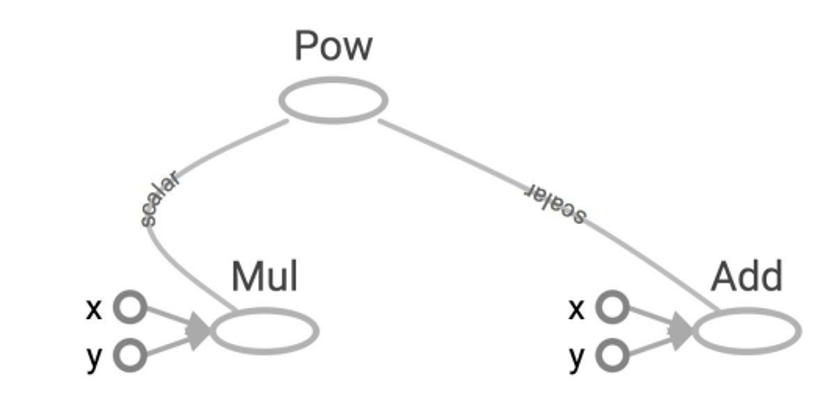
\includegraphics[width=\linewidth,keepaspectratio]{drawgraph}
\end{center}
\end{minipage}
}
\begin{itemize}
\item When $op3$ is run, then it goes back to all the dependent nodes till it finds are the data specified/necessary to make this symbolic calculation concrete and then executes those traced nodes.
\item Multiple nodes can be evaluated in a sing $run$ by passing [] array

\end{itemize}
\end{frame}


%%%%%%%%%%%%%%%%%%%%%%%%%%%%%%%%%%%%%%%%%%%%%%%%%%%
\begin{frame}[fragile] \frametitle{Untraced Nodes}

\adjustbox{valign=t}{
\begin{minipage}{0.45\linewidth}
\begin{lstlisting}
x = 2
y = 3
op1 = tf.add(x, y)
op2 = tf.mul(x, y)
useless = tf.mul(x, op1)
op3 = tf.pow(op2, op1)
with tf.Session() as sess:
    op3 = sess.run(op3)

\end{lstlisting}
\end{minipage}
}
\hfill
\adjustbox{valign=t}{
\begin{minipage}{0.4\linewidth}
\begin{center}
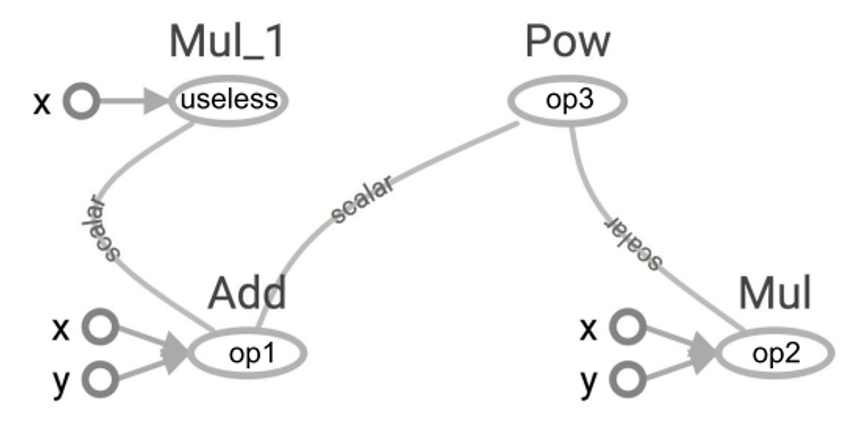
\includegraphics[width=\linewidth,keepaspectratio]{untracednodes}
\end{center}
\end{minipage}
}
\begin{itemize}
\item From output node, tracking goes till all the inputs are satisfied.
\item Nodes which are not in this path are not evaluated.
\item For $op3$, $op1$ and $op2$ are needed but not the $useless$ so not evaluated
\end{itemize}
\end{frame}




%%%%%%%%%%%%%%%%%%%%%%%%%%%%%%%%%%%%%%%%%%%%%%%%%%%
\begin{frame}[fragile] \frametitle{Parallelization}

\adjustbox{valign=t}{
\begin{minipage}{0.45\linewidth}
\begin{itemize}
\item Internally graph is broken into several chunks and run them parallelly across multiple CPUs, GPUs, or devices
\item Device can be specified as well
\end{itemize}

\end{minipage}
}
\hfill
\adjustbox{valign=t}{
\begin{minipage}{0.4\linewidth}
\begin{center}
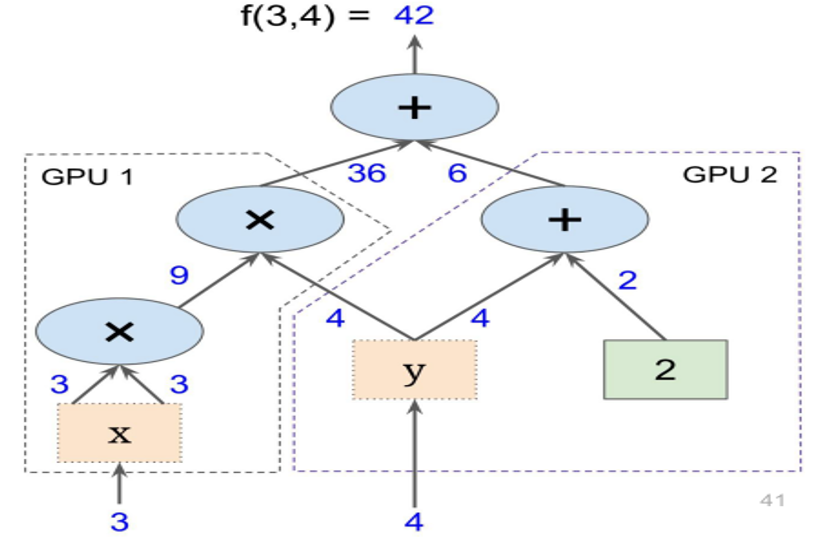
\includegraphics[width=\linewidth,keepaspectratio]{parallelgraph}
\end{center}
\end{minipage}
}
\begin{lstlisting}
# Creates a graph.
with tf.device('/gpu:2'):
	a = tf.constant([1.0], name='a')
	b = tf.constant([1.0], name='b')
	c = tf.matmul(a, b)
\end{lstlisting}
\end{frame}

%%%%%%%%%%%%%%%%%%%%%%%%%%%%%%%%%%%%%%%%%%%%%%%%%%%
\begin{frame}[fragile] \frametitle{Multiple Graphs}

\begin{itemize}
\item Generally, default graph run in the session is sufficient. 
\item No need to create multiple graphs. 
\item That would need multiple sessions.
\begin{lstlisting}
g = tf.Graph()

with g.as_default():
    x = tf.add(3, 5)

sess = tf.Session(graph=g)

with tf.Session() as sess:
    sess.run(x)
\end{lstlisting}
\end{itemize}
\end{frame}


%%%%%%%%%%%%%%%%%%%%%%%%%%%%%%%%%%%%%%%%%%%%%%%%%%%
\begin{frame}[fragile] \frametitle{Why Graphs?}
\begin{itemize}
\item Save computation (only run subgraphs that are traced for a particular run-request)
\item Break computation into small, differential pieces 
\item Facilitate distributed computation, spread the work across multiple CPUs, GPUs, or devices
\item Many common machine learning models are commonly taught and visualized as directed graphs already
\end{itemize}
\end{frame}


%%%%%%%%%%%%%%%%%%%%%%%%%%%%%%%%%%%%%%%%%%%%%%%%%%%
\begin{frame}[fragile] \frametitle{First program in TensorFlow}
\begin{itemize}
\item Simple addition
\begin{lstlisting}
import tensorflow as tf
a = tf.constant(2)
b = tf.constant(3)
x = tf.add(a, b)
with tf.Session() as sess:
    print(sess.run(x))
\end{lstlisting}
\item To see in tensor board
\begin{lstlisting}
with tf.Session() as sess:
	# add this line to use TensorBoard. 
	writer = tf.summary.FileWriter('./graphs, sess.graph) 
	print sess.run(x)
writer.close() # close the writer when you're done using it
\end{lstlisting}
\item To run
\begin{lstlisting}
$ tensorboard --logdir="./graphs" --port 6006
\end{lstlisting}
\item View http://localhost:6006/
\end{itemize}
\end{frame}


%%%%%%%%%%%%%%%%%%%%%%%%%%%%%%%%%%%%%%%%%%%%%%%%%%%
\begin{frame}[fragile] \frametitle{TensorBoard}
\begin{itemize}
\item See Graphs
\begin{center}
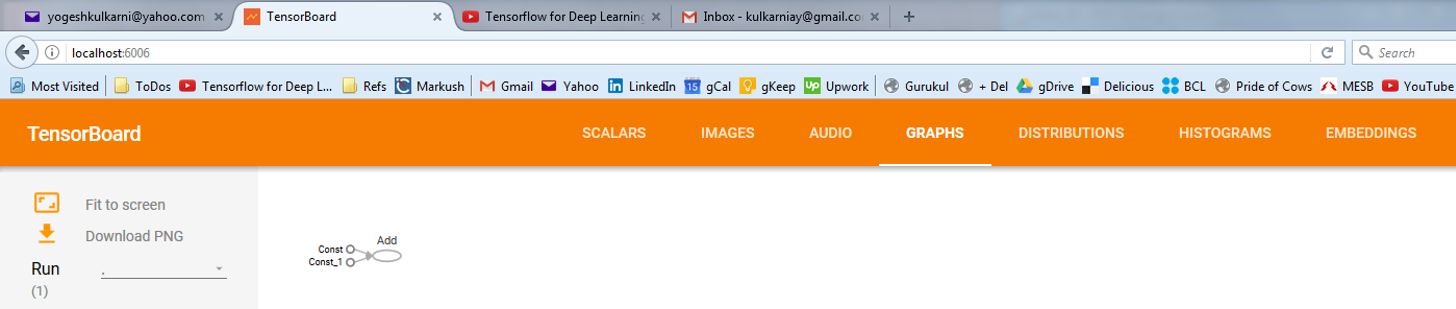
\includegraphics[width=0.8\linewidth,keepaspectratio]{tensorboard}
\end{center}
\item For code
\begin{lstlisting}
a = tf.constant(2, name=``a'')
b = tf.constant(3, name=``b'')
x = tf.add(a, b, name=``add'')
\end{lstlisting}
\end{itemize}
\end{frame}


%%%%%%%%%%%%%%%%%%%%%%%%%%%%%%%%%%%%%%%%%%%%%%%%%%%
\begin{frame}[fragile] \frametitle{Constants}
\begin{itemize}
\item Definition
\begin{lstlisting}
tf.constant(value, dtype=None,shape=None,name='Const', verify_shape=False)
\end{lstlisting}
\item Usage
\begin{lstlisting}
a = tf.constant([2, 2], name=``a'')
b = tf.constant([[0, 1], [2, 3]], name=``b'')
\end{lstlisting}
\item Tensors filled with specific values
\begin{lstlisting}
tf.zeros([2, 3], tf.int32) ==> [[0, 0, 0], [0, 0, 0]]
\end{lstlisting}
\item To create a tensor of shape and type as the input\_tensor but all elements are zeros. Values are immaterial but shape is.
\begin{lstlisting}
# input_tensor is [0, 1], [2, 3], [4, 5]]
tf.zeros_like(input_tensor) ==> [[0, 0], [0, 0], [0, 0]]
\end{lstlisting}
\item Similarly for $ones$
\end{itemize}
\end{frame}

%%%%%%%%%%%%%%%%%%%%%%%%%%%%%%%%%%%%%%%%%%%%%%%%%%%
\begin{frame}[fragile] \frametitle{Constants as Sequences}
\begin{itemize}
\item Definition
\begin{lstlisting}
tf.linspace(start, stop, num, name=None) # diff from np.linspace
tf.linspace(10.0, 13.0, 4) ==> [10.0 11.0 12.0 13.0]

tf.range(start, limit=None, delta=1, dtype=None, name='range')
# 'start' is 3, 'limit' is 18, 'delta' is 3
tf.range(start, limit, delta) ==> [3, 6, 9, 12, 15]

# 'limit' is 5
tf.range(limit) ==> [0, 1, 2, 3, 4]
\end{lstlisting}
\item Tensor objects are not iterable
\begin{lstlisting}
for _ in tf.range(4): # TypeError
\end{lstlisting}
\end{itemize}
\end{frame}


%%%%%%%%%%%%%%%%%%%%%%%%%%%%%%%%%%%%%%%%%%%%%%%%%%%
\begin{frame}[fragile] \frametitle{Random numbers Sequences}
\begin{itemize}
\item Definition
\begin{lstlisting}
tf.random_normal(shape, mean=0.0, stddev=1.0, dtype=tf.float32, seed=None, name=None)
tf.truncated_normal(shape, mean=0.0,stddev=1.0,dtype=tf.float32, seed=None, name=None)
tf.random_uniform(shape,minval=0, maxval=None,dtype=tf.float32, seed=None, name=None)
tf.random_shuffle(value, seed=None, name=None)
tf.random_crop(value, size, seed=None, name=None)
tf.multinomial(logits, num_samples, seed=None, name=None)
tf.random_gamma(shape, alpha, beta=None,dtype=tf.float32,seed=None, name=None)
\end{lstlisting}
\item To have same random pattern, set seed as
\begin{lstlisting}
tf.set_random_seed(seed)
\end{lstlisting}
\end{itemize}
\end{frame}

%%%%%%%%%%%%%%%%%%%%%%%%%%%%%%%%%%%%%%%%%%%%%%%%%%%
\begin{frame}[fragile] \frametitle{Operations}
\begin{center}
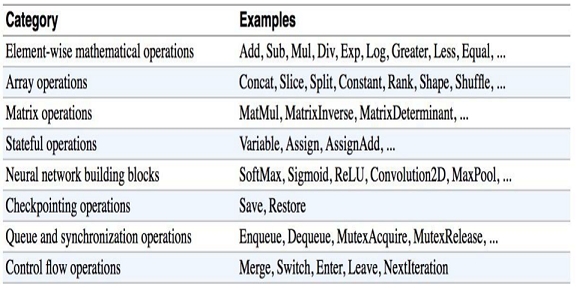
\includegraphics[width=0.8\linewidth,keepaspectratio]{ops}
\end{center}
\begin{lstlisting}
a = tf.constant([3, 6])
b = tf.constant([2, 2])
tf.add(a, b) # >> [5 8]
tf.add_n([a, b, b]) # >> [7 10]. Equivalent to a + b + b
\end{lstlisting}
\end{frame}


%%%%%%%%%%%%%%%%%%%%%%%%%%%%%%%%%%%%%%%%%%%%%%%%%%%
\begin{frame}[fragile] \frametitle{TensorFlow Data Types}
\begin{itemize}
\item TensorFlow takes Python natives types: boolean, int, float, strings
\item 0-d tensor, or $scalar$ 
\item 1-d tensor, or $vector$
\item 2x2 tensor, or $matrix$
\end{itemize}
\begin{lstlisting}
t_0 = 19 
tf.zeros_like(t_0) # ==> 0
tf.ones_like(t_0) # ==> 1
t_1 = ['apple', 'peach', 'banana']
tf.zeros_like(t_1) # ==> ['' '' '']
tf.ones_like(t_1) # ==> TypeError: Expected string, got 1 as 'int' instead.
t_2 = [[True, False, False],
       [False, False, True],
       [False, True, False]] 
\end{lstlisting}
\end{frame}

%%%%%%%%%%%%%%%%%%%%%%%%%%%%%%%%%%%%%%%%%%%%%%%%%%%
\begin{frame}[fragile] \frametitle{TensorFlow vs Numpy Data Types}
\begin{itemize}
\item TensorFlow integrates seamlessly with NumPy
\item Can pass numpy types to TensorFlow ops
\begin{lstlisting}
tf.int32 == np.int32 # True
tf.ones([2, 2], np.float32) #  [[1.0 1.0], [1.0 1.0]]
\end{lstlisting}
\item But, do not use Python native types for tensors because TensorFlow has to infer Python type
\item Even not numpy, as they may become incompatible in future
\item Use constants for primitive types
\item Use variables, as big constants may make graph loading expensive
\item Constants are stored in graph definition whereas variables are allocated by the session.
\end{itemize}

\end{frame}


%%%%%%%%%%%%%%%%%%%%%%%%%%%%%%%%%%%%%%%%%%%%%%%%%%%
\begin{frame}[fragile] \frametitle{Variables}
When creating a variable, you can set an initial value explicitly, or you can use an initializer (like a distribution):
\begin{lstlisting}
g = tf.Graph()
with g.as_default():
  # Create a variable with the initial value 3.
  v = tf.Variable([3])

  # Create a variable of shape [1], with a random initial value,
  # sampled from a normal distribution with mean 1 and standard deviation 0.35.
  w = tf.Variable(tf.random_normal([1], mean=1.0, stddev=0.35))
\end{lstlisting}
\end{frame}


%%%%%%%%%%%%%%%%%%%%%%%%%%%%%%%%%%%%%%%%%%%%%%%%%%%
\begin{frame}[fragile] \frametitle{Variables}
One peculiarity of TensorFlow is that variable initialization is not automatic. For example, the following block will cause an error:
\begin{lstlisting}
with g.as_default():
  with tf.Session() as sess:
    try:
      v.eval()
    except tf.errors.FailedPreconditionError as e:
      print "Caught expected error: ", e
\end{lstlisting}
\end{frame}

%%%%%%%%%%%%%%%%%%%%%%%%%%%%%%%%%%%%%%%%%%%%%%%%%%%
\begin{frame}[fragile] \frametitle{Variables}
The easiest way to initialize a variable is to call global\_variables\_initializer. Note the use of Session.run(), which is roughly equivalent to eval().
\begin{lstlisting}
with g.as_default():
  with tf.Session() as sess:
    initialization = tf.global_variables_initializer()
    sess.run(initialization)
    # Now, variables can be accessed normally, and have values assigned to them.
    print v.eval()
    print w.eval()
\end{lstlisting}
\end{frame}

%%%%%%%%%%%%%%%%%%%%%%%%%%%%%%%%%%%%%%%%%%%%%%%%%%%
\begin{frame}[fragile] \frametitle{Variables}
Once initialized, variables will maintain their value within the same session (however, when starting a new session, you will need to re-initialize them):
\begin{lstlisting}
with g.as_default():
  with tf.Session() as sess:
    sess.run(tf.global_variables_initializer())
    # These three prints will print the same value.
    print w.eval()
    print w.eval()
    print w.eval()
\end{lstlisting}
\end{frame}

%%%%%%%%%%%%%%%%%%%%%%%%%%%%%%%%%%%%%%%%%%%%%%%%%%%
\begin{frame}[fragile] \frametitle{Variables}
To change the value of a variable, use the assign op. Note that simply creating the assign op will not have any effect. As with initialization, you have to run the assignment op to update the variable value:
\begin{lstlisting}
with g.as_default():
  with tf.Session() as sess:
    sess.run(tf.global_variables_initializer())
    # This should print the variable's initial value.
    print v.eval()

    assignment = tf.assign(v, [7])
    # The variable has not been changed yet!
    print v.eval()

    # Execute the assignment op.
    sess.run(assignment)
    # Now the variable is updated.
    print v.eval()
\end{lstlisting}
\end{frame}


%%%%%%%%%%%%%%%%%%%%%%%%%%%%%%%%%%%%%%%%%%%%%%%%%%%
\begin{frame}[fragile] \frametitle{Variables}

\begin{lstlisting}
# create variable a with scalar value
a = tf.Variable(2, name=``scalar'') 
# create variable b as a vector
b = tf.Variable([2, 3], name=``vector'') 
# create variable c as a 2x2 matrix
c = tf.Variable([[0, 1], [2, 3]], name=``matrix'') 
# create variable W as 784 x 10 tensor, filled with zeros
W = tf.Variable(tf.zeros([784,10]))
\end{lstlisting}
\begin{itemize}
\item Why $tf.constant$ but $tf.Variable$ and not $tf.variable$? 
\item \pause $tf.Variable$ is a class, but $tf.constant$ is an op

\end{itemize}

\end{frame}


%%%%%%%%%%%%%%%%%%%%%%%%%%%%%%%%%%%%%%%%%%%%%%%%%%%
\begin{frame}[fragile] \frametitle{Variables}
\begin{itemize}
\item $tf.Variable$ holds several ops:
\begin{lstlisting}
x = tf.Variable(...) 
x.initializer # init op
x.value() # read op
x.assign(...) # write op
x.assign_add(...) # and more
\end{lstlisting}
\item You have to initialize your variables
\begin{lstlisting}
init = tf.global_variables_initializer()
with tf.Session() as sess:
	sess.run(init)
\end{lstlisting}
\item Also
\begin{lstlisting}
W = tf.Variable(tf.zeros([784,10]))
with tf.Session() as sess:
    sess.run(W.initializer)
\end{lstlisting}
\end{itemize}

\end{frame}


%%%%%%%%%%%%%%%%%%%%%%%%%%%%%%%%%%%%%%%%%%%%%%%%%%%
\begin{frame}[fragile] \frametitle{Eval on a Variable}
\begin{itemize}
\item Printing variable will print the Tensor datatype
\begin{lstlisting}
# W is a random 700 x 100 variable object
W = tf.Variable(tf.truncated_normal([700, 10]))
with tf.Session() as sess:
	sess.run(W.initializer)
       print(W)
>> Tensor("Variable/read:0", shape=(700, 10), dtype=float32)
\end{lstlisting}
\item To print its value, use $eval()$
\begin{lstlisting}
with tf.Session() as sess:
    sess.run(W.initializer)
    print(W.eval())
\end{lstlisting}
\end{itemize}

\end{frame}


%%%%%%%%%%%%%%%%%%%%%%%%%%%%%%%%%%%%%%%%%%%%%%%%%%%
\begin{frame}[fragile] \frametitle{Assign on a Variable}

\begin{lstlisting}
W = tf.Variable(10)
W.assign(100)
with tf.Session() as sess:
	sess.run(W.initializer)
	print(W.eval()) # gives 10
\end{lstlisting}

$W.assign(100)$ doesn't assign the value $100$ to $W$. It creates an assign op, and that op needs to be run to take effect.

\begin{lstlisting}
W = tf.Variable(10)
assign_op = W.assign(100)
with tf.Session() as sess:
	sess.run(W.initializer)
	sess.run(assign_op) # above initialization is unnecessary as assign does it
	print(W.eval()) # gives 100
\end{lstlisting}

\end{frame}


%%%%%%%%%%%%%%%%%%%%%%%%%%%%%%%%%%%%%%%%%%%%%%%%%%%
\begin{frame}[fragile] \frametitle{Assign on a Variable and running many times}

\begin{lstlisting}
my_var = tf.Variable(2, name=``my_var'') 
my_var_times_two = my_var.assign(2 * my_var)
with tf.Session() as sess:
	sess.run(my_var.initializer)
	sess.run(my_var_times_two) # assigns 4
	sess.run(my_var_times_two) # assigns 8
	sess.run(my_var_times_two) # assigns 16
sess1.close()
sess2.close()
\end{lstlisting}

It assign $2 * my\_var$ to a every time $my\_var\_times\_two$ is fetched.


\begin{lstlisting}
W = tf.Variable(10)
assign_op = W.assign(100)
with tf.Session() as sess:
	sess.run(W.initializer)
	sess.run(assign_op) # above initialization is uncessary as assign does it
	print(W.eval()) # gives 100
\end{lstlisting}

\end{frame}

%%%%%%%%%%%%%%%%%%%%%%%%%%%%%%%%%%%%%%%%%%%%%%%%%%%
\begin{frame}[fragile] \frametitle{Exercise: Simulate 10 rolls of two dice.}
\begin{itemize}
\item Create a dice simulation, which generates a 10x3 2-D tensor in which:
\begin{itemize}
\item Columns 1 and 2 each hold one throw of one die.
\item Column 3 holds the sum of Columns 1 and 2 on the same row.
\end{itemize}
\item For example, the first row might have the following values:
\begin{itemize}
\item Column 1 holds 4
\item Column 2 holds 3
\item Column 3 holds 7
\end{itemize}
\end{itemize}
\end{frame}




%%%%%%%%%%%%%%%%%%%%%%%%%%%%%%%%%%%%%%%%%%%%%%%%%%%
\begin{frame}[fragile] \frametitle{Session scope for variables}

\begin{lstlisting}
W = tf.Variable(10)
sess1 = tf.Session()
sess2 = tf.Session()
sess1.run(W.initializer)
sess2.run(W.initializer)
print sess1.run(W.assign_add(10)) # assigns 20
print sess2.run(W.assign_sub(2)) # assigns 8
sess1.close()
sess2.close()
\end{lstlisting}

Each session maintains its own copy of variable
\end{frame}

%%%%%%%%%%%%%%%%%%%%%%%%%%%%%%%%%%%%%%%%%%%%%%%%%%%
\begin{frame}[fragile] \frametitle{Using variable to initialize other}
\begin{itemize}
\item Want to declare $U = 2 * W$

\begin{lstlisting}
# W is a random 700 x 100 tensor
W = tf.Variable(tf.truncated_normal([700, 10]))
U = tf.Variable(2 * W)
\end{lstlisting}
\item Not so safe (but quite common)
\begin{lstlisting}
# W is a random 700 x 100 tensor
W = tf.Variable(tf.truncated_normal([700, 10]))
U = tf.Variable(2 * W.intialized_value()) 
\end{lstlisting}
\item Ensure that $W$ is initialized before its value is used to initialize $U$, Safe.

\end{itemize}

\end{frame}


%%%%%%%%%%%%%%%%%%%%%%%%%%%%%%%%%%%%%%%%%%%%%%%%%%%
\begin{frame}[fragile] \frametitle{Session vs InteractiveSession}
Difference is an InteractiveSession makes itself the default

\begin{lstlisting}
sess = tf.InteractiveSession()
a = tf.constant(5.0)
b = tf.constant(6.0)
c = a * b
# We can just use 'c.eval()' without specifying the context 'sess'
print(c.eval())
sess.close()
\end{lstlisting}

\end{frame}

%%%%%%%%%%%%%%%%%%%%%%%%%%%%%%%%%%%%%%%%%%%%%%%%%%%
\begin{frame}[fragile] \frametitle{Control Dependencies/Execution order}
Defines which ops should be run first
\begin{lstlisting}
# your graph g have 5 ops: a, b, c, d, e
with g.control_dependencies([a, b, c]):
	# 'd' and 'e' will only run after 'a', 'b', and 'c' have executed.
	d = 
	e = 
\end{lstlisting}

\end{frame}

%%%%%%%%%%%%%%%%%%%%%%%%%%%%%%%%%%%%%%%%%%%%%%%%%%%
\begin{frame}[fragile] \frametitle{Placeholders}
\begin{itemize}
\item Graph can be assembled without knowing some of the (input) values
\item You (can) always define a function, in such symbolic way.
\item $f(x, y) = x*2 + y$ without knowing value of $x$ or $y$. 
\item $x$, $y$ are placeholders for the actual values.
\item They are fed into graph at $run$ via dictionary.
\begin{lstlisting}
# create a placeholder float 32-bit, shape is a vector of 3 elements
a = tf.placeholder(tf.float32, shape=[3])
\end{lstlisting}
\item Special note: dictionary syntax used here is not as in Python, where keys are strings like $a$, but direct variable is the key.
\end{itemize}

\end{frame}

%%%%%%%%%%%%%%%%%%%%%%%%%%%%%%%%%%%%%%%%%%%%%%%%%%%
\begin{frame}[fragile] \frametitle{Feed the Placeholders}
\begin{lstlisting}
a = tf.placeholder(tf.float32, shape=[3])
b = tf.constant([5, 5, 5], tf.float32)
c = a + b  # Short for tf.add(a, b)
with tf.Session() as sess:
	print(sess.run(c, {a: [1, 2, 3]})) # a is the placeholder defined
\end{lstlisting}
$ [6, 7, 8]$
\begin{itemize}
\item Shape can be $None$, which concreted defined at feeding
\item Values can be fed, via dictionary, into ops even if they are not placeholders, during $run$. Helpful for debugging.
\end{itemize}

\end{frame}


%%%%%%%%%%%%%%%%%%%%%%%%%%%%%%%%%%%%%%%%%%%%%%%%%%%
\begin{frame}[fragile] \frametitle{What's lazy loading?}
Defer creating/initializing an object until it is needed


\adjustbox{valign=t}{
\begin{minipage}{0.45\linewidth}
\begin{itemize}
\item Normal loading:
\item Node $Add$ added once to the graph definition
\end{itemize}
\begin{lstlisting}
x = tf.Variable(10, name='x')
y = tf.Variable(20, name='y')
z = tf.add(x, y) # EARLY
with tf.Session() as sess:
	sess.run(tf.global_variables_initializer())
	for _ in range(10):
		sess.run(z)
\end{lstlisting}
\end{minipage}
}
\hfill
\adjustbox{valign=t}{
\begin{minipage}{0.45\linewidth}
\begin{itemize}
\item Lazy loading:

\item Node $Add$ added 10 times to the graph
\end{itemize}
\begin{lstlisting}
x = tf.Variable(10, name='x')
y = tf.Variable(20, name='y')
with tf.Session() as sess:
	sess.run(tf.global_variables_initializer())
	for _ in range(10):
		sess.run(tf.add(x, y))
\end{lstlisting}
\end{minipage}
}

\end{frame}



%%%%%%%%%%%%%%%%%%%%%%%%%%%%%%%%%%%%%%%%%%%%%%%%%%%
\begin{frame}[fragile] \frametitle{Loading differences}
\adjustbox{valign=t}{
\begin{minipage}{0.45\linewidth}
\begin{itemize}
\item Problems with Lazy loading:
\item Imagine you want to compute an op thousands of times!
\item Your graph gets bloated
\item Slow to load
\item Expensive to pass around
\item Most common TF non-bug bugs 
\end{itemize}
\end{minipage}
}
\hfill
\adjustbox{valign=t}{
\begin{minipage}{0.45\linewidth}
\begin{itemize}
\item Solution:
\item Separate definition of ops from computing/running ops 
\item Use Python @property to ensure function is also loaded once the first time it is called
\end{itemize}
\end{minipage}
}

\end{frame}

%%%%%%%%%%%%%%%%%%%%%%%%%%%%%%%%%%%%%%%%%%%%%%%%%%%
\begin{frame}[fragile] \frametitle{Simple Program: Linear Regression}
\begin{itemize}
\item Model relationship between a scalar dependent variable $y$ and independent (many) variables $X$
\item City of Chicago:
\begin{itemize}
\item $X$: number of incidents of fire
\item $Y$: number of incidents of theft
\end{itemize}
\item Want: Predict $Y$ from $X$
\item Model:
\begin{itemize}
\item $w * X + b$
\item $(Y - Y_predicted) 2$
\end{itemize}
\end{itemize}
\end{frame}



%%%%%%%%%%%%%%%%%%%%%%%%%%%%%%%%%%%%%%%%%%%%%%%%%%%
\begin{frame}[fragile] \frametitle{Simple Program: Linear Regression}
\adjustbox{valign=t}{
\begin{minipage}{0.45\linewidth}
\begin{itemize}
\item Phase 1: Assemble our graph
\begin{itemize}
\item Read in data
\item Create placeholders for inputs and labels
\item Create weight and bias
\item  Specify model 
\item Specify loss function 
\item Create optimizer 
\end{itemize}
\end{itemize}
\end{minipage}
}
\hfill
\adjustbox{valign=t}{
\begin{minipage}{0.45\linewidth}
\begin{itemize}
\item Phase 2: Train model
\begin{itemize}
\item Initialize variables
\item Run optimizer op (with data fed into placeholders for inputs and labels)
\end{itemize}
\item See your model in TensorBoard
\begin{itemize}
\item Write graph to file
\item See it in Tensorboard
\end{itemize}
\end{itemize}
\end{minipage}
}

\end{frame}


%%%%%%%%%%%%%%%%%%%%%%%%%%%%%%%%%%%%%%%%%%%%%%%%%%%
\begin{frame}[fragile] \frametitle{Simple Regression Graph}
\begin{center}
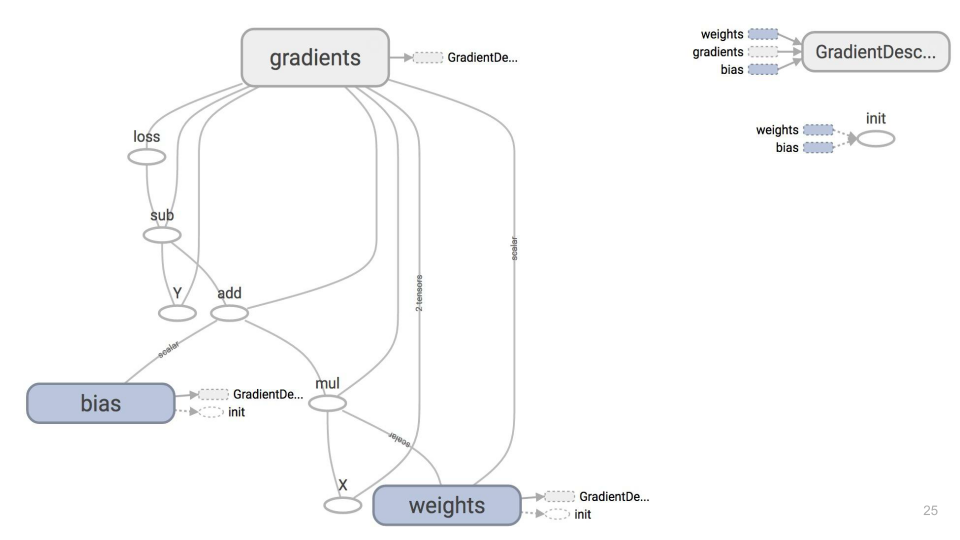
\includegraphics[width=\linewidth,keepaspectratio]{simplregr}
\end{center}
\end{frame}


%%%%%%%%%%%%%%%%%%%%%%%%%%%%%%%%%%%%%%%%%%%%%%%%%%%
\begin{frame}[fragile] \frametitle{Simple Regression Code}
\begin{center}
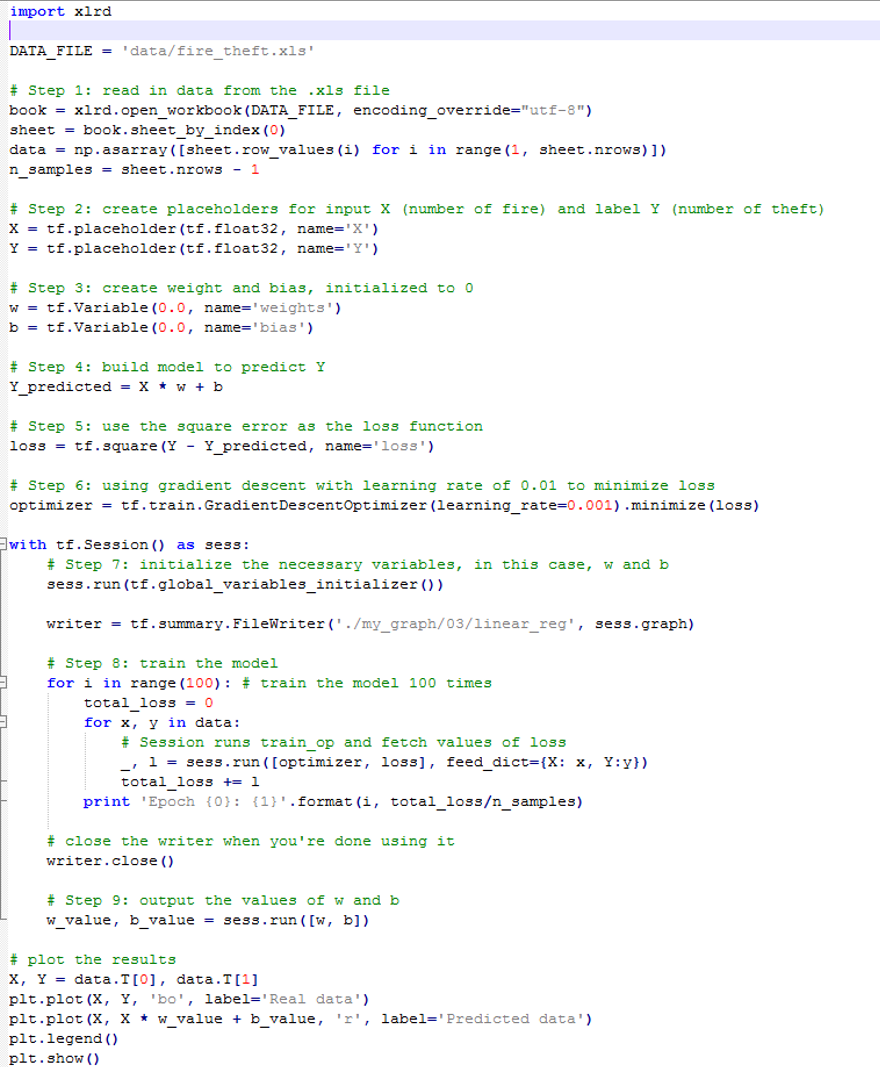
\includegraphics[width=0.8\linewidth,keepaspectratio]{simplregrcode}
\end{center}
\end{frame}


%%%%%%%%%%%%%%%%%%%%%%%%%%%%%%%%%%%%%%%%%%%%%%%%%%%
\begin{frame}[fragile] \frametitle{Simple Regression Results}
\begin{center}
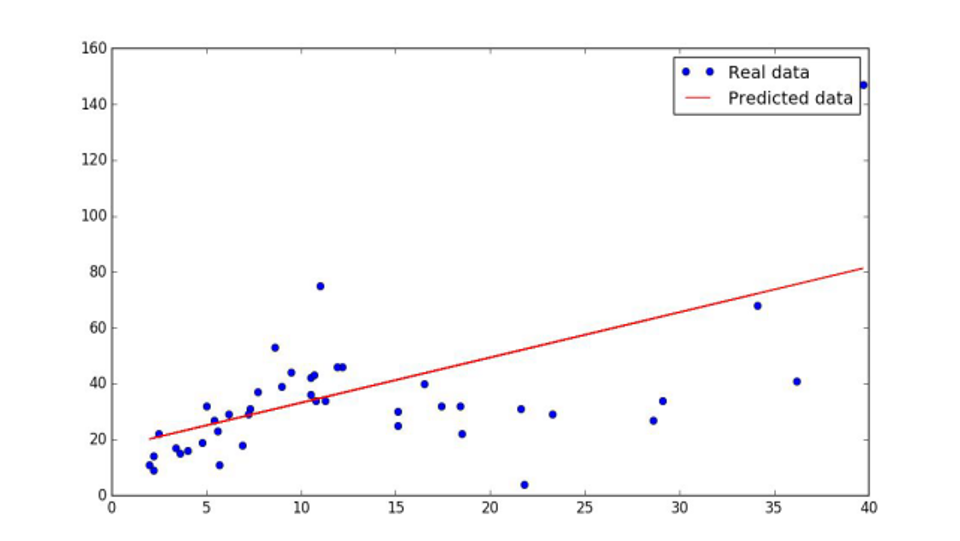
\includegraphics[width=\linewidth,keepaspectratio]{simplregrresults}
\end{center}
\end{frame}



%%%%%%%%%%%%%%%%%%%%%%%%%%%%%%%%%%%%%%%%%%%%%%%%%%%
\begin{frame}[fragile] \frametitle{How session knows which variables to update?}
\begin{itemize}
\item $W$ and $b$ needs to be updated. But how session knows that?
\begin{lstlisting}
optimizer = tf.train.GradientDescentOptimizer(learning_rate=0.001).minimize(loss)
_, l = sess.run([optimizer, loss], feed_dict={X: x, Y:y})
\end{lstlisting}
\item Session looks at all trainable variables that loss depends on
\item Optimizer depends on loss and loss depends on $Y_{pred}$, which depends on $W$ and $b$, thus $W$ and $b$ are updated.
\end{itemize}

\end{frame}



%%%%%%%%%%%%%%%%%%%%%%%%%%%%%%%%%%%%%%%%%%%%%%%%%%%
\begin{frame}[fragile] \frametitle{List of Optimizers}
\begin{lstlisting}
tf.train.GradientDescentOptimizer
tf.train.AdagradOptimizer
tf.train.MomentumOptimizer
tf.train.AdamOptimizer
tf.train.ProximalGradientDescentOptimizer
tf.train.ProximalAdagradOptimizer
tf.train.RMSPropOptimizer
# And more
\end{lstlisting}
\end{frame}



%%%%%%%%%%%%%%%%%%%%%%%%%%%%%%%%%%%%%%%%%%%%%%%%%%%
\begin{frame}[fragile] \frametitle{Simple Program: MNIST as Logistic Regression}

\adjustbox{valign=t}{
\begin{minipage}{0.45\linewidth}
\begin{itemize}
\item MNIST: Images of $28x28$ array, flattened as 1-d tensor of size $784$
\begin{center}
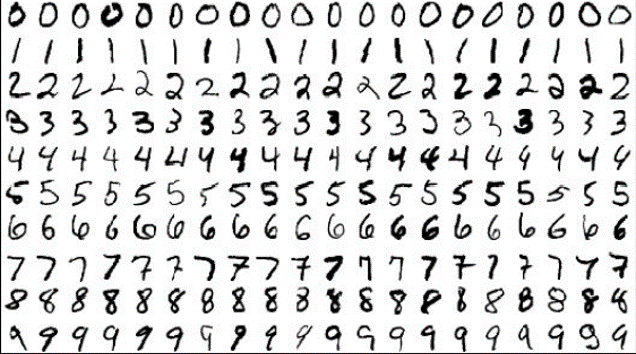
\includegraphics[width=\linewidth,keepaspectratio]{mnistdigits}
\end{center}
\item $X$: image of a handwritten digit
\item $Y$: the digit value
\item Goal: Recognize digits
\end{itemize}
\end{minipage}
}
\hfill
\adjustbox{valign=t}{
\begin{minipage}{0.45\linewidth}
\begin{itemize}
\item Model
\begin{itemize}
\item $logits = X * w + b$
\item $Y_{predicted} = softmax(logits)$
\item $loss = cross\_entropy(Y, Y_{predicted})$
\end{itemize}
\item Batch
\begin{lstlisting}
X = tf.placeholder(tf.float32, [batch_size, 784], name=``image'') 
Y = tf.placeholder(tf.float32, [batch_size, 10], name=``label'')
\end{lstlisting}
\end{itemize}
\end{minipage}
}

\end{frame}


%%%%%%%%%%%%%%%%%%%%%%%%%%%%%%%%%%%%%%%%%%%%%%%%%%%
\begin{frame}[fragile] \frametitle{How to find specific gradients?}
\begin{itemize}
\item  Derivative of y with respect to each tensor in the list [xs]
\begin{lstlisting}
x = tf.Variable(2.0)
y = 2.0 * (x ** 3)
z = 3.0 + y ** 2
grad_z = tf.gradients(z, [x, y])
with tf.Session() as sess:
	sess.run(x.initializer)
	print sess.run(grad_z) #[768.0, 32.0]
# 768 is the gradient of z with respect to x, 32 with respect to y
\end{lstlisting}
\item Vanishing/Exploding gradients: Can become very high ($NaN$) or goes to zero, and fails to compute minima.
\end{itemize}
\end{frame}


%%%%%%%%%%%%%%%%%%%%%%%%%%%%%%%%%%%%%%%%%%%%%%%%%%%
\begin{frame}[fragile] \frametitle{How to structure code?}

\adjustbox{valign=t}{
\begin{minipage}{0.45\linewidth}
\begin{itemize}
\item Object Oriented
\item  Base Model class
\begin{itemize}
\item  Load data
\item  Create Place holder
\item  Add loss
\item  Add Optimizer
\item  Run Epochs
\item Predict
\end{itemize}
\item A word2vec skipgram model is shown on right
\end{itemize}
\end{minipage}
}
\hfill
\adjustbox{valign=t}{
\begin{minipage}{0.45\linewidth}
\begin{lstlisting}
class SkipGramModel:
    def __init__(self, params):
        pass
    def _create_placeholders(self):
        pass
    def _create_embedding(self):
        pass
    def _create_loss(self):
        pass
    def _create_optimizer(self):
        pass
\end{lstlisting}
\end{minipage}
}

\end{frame}


%%%%%%%%%%%%%%%%%%%%%%%%%%%%%%%%%%%%%%%%%%%%%%%%%%%
\begin{frame}[fragile] \frametitle{Intermittent saving}

\adjustbox{valign=t}{
\begin{minipage}{0.45\linewidth}
\begin{itemize}
\item $tf.train.Saver$ saves graph's variables in binary files
\item Saves session (graph's variables)
\item Save parameters after 1000 steps
\item Each saved step is a checkpoint
\item by $global\_step=model.global\_step$
\item For every op, global step is incremented automatically
\end{itemize}
\end{minipage}
}
\hfill
\adjustbox{valign=t}{
\begin{minipage}{0.45\linewidth}
\begin{lstlisting}
# define model
# create a saver object
saver = tf.train.Saver()
# launch a session to compute the graph
with tf.Session() as sess:
    # actual training loop
    for step in range(training_steps): 
        sess.run([optimizer])
        if (step + 1) \% 1000==0:
            saver.save(sess, 'checkpoint_directory/model_name', global_step=model.global_step)
\end{lstlisting}
\end{minipage}
}

\end{frame}


%%%%%%%%%%%%%%%%%%%%%%%%%%%%%%%%%%%%%%%%%%%%%%%%%%%
\begin{frame}[fragile] \frametitle{Restoring Saved model}

\adjustbox{valign=t}{
\begin{minipage}{0.45\linewidth}
\begin{itemize}
\item Restore the latest checkpoint
\item Checkpoint keeps track of the latest checkpoint
\item Safeguard to restore checkpoints only when there are checkpoint
\item If model is running for hours, put checkpoint after each hour or so.
\end{itemize}
\end{minipage}
}
\hfill
\adjustbox{valign=t}{
\begin{minipage}{0.45\linewidth}
\begin{lstlisting}
ckpt = tf.train.get_checkpoint_state(os.path.dirname('checkpoints/checkpoint'))
if ckpt and ckpt.model_checkpoint_path:
     saver.restore(sess, ckpt.model_checkpoint_path)
\end{lstlisting}
\end{minipage}
}

\end{frame}


%%%%%%%%%%%%%%%%%%%%%%%%%%%%%%%%%%%%%%%%%%%%%%%%%%%
\begin{frame}[fragile] \frametitle{Summarizing model}

\adjustbox{valign=t}{
\begin{minipage}{0.45\linewidth}
\begin{itemize}
\item Summarise upon events during training.
\begin{itemize}
\item $tf.summary.scalar (``loss'')$
\item $tf.summary.histogram$
\item $tf.summary.image$
\end{itemize}
\item Step 1: create summaries
\item Step 2: run them
\item Step 3: write summaries to file
\item See summaries on TensorBoard
\end{itemize}
\end{minipage}
}
\hfill
\adjustbox{valign=t}{
\begin{minipage}{0.45\linewidth}
\begin{lstlisting}
with tf.name_scope(``summaries''):
    tf.summary.scalar(``loss'', self.loss
    tf.summary.scalar(``accuracy'', self.accuracy)            
    tf.summary.histogram(``histogram loss'', self.loss)
    # merge them all
    self.summary_op = tf.summary.merge_all()
loss_batch, _, summary = sess.run([model.loss, model.optimizer, 
model.summary_op], 
feed_dict=feed_dict)
writer.add_summary(summary, global_step=step)
\end{lstlisting}
\end{minipage}
}

\end{frame}


%%%%%%%%%%%%%%%%%%%%%%%%%%%%%%%%%%%%%%%%%%%%%%%%%%%
\begin{frame}[fragile] \frametitle{Data readers}

\adjustbox{valign=t}{
\begin{minipage}{0.45\linewidth}
\begin{itemize}
\item Problem with feed\_dict?
\item Slow when client and workers are on different machines
\item Readers allow us to load data directly into the worker process.
\item Ops that return different values every time you call them
\item Think Python's generator
\item Different Readers for different file types
\end{itemize}
\end{minipage}
}
\hfill
\adjustbox{valign=t}{
\begin{minipage}{0.45\linewidth}
\begin{lstlisting}
tf.TextLineReader
Outputs the lines of a file delimited by newlines
E.g. text files, CSV files
tf.FixedLengthRecordReader
Outputs the entire file when all files have same fixed lengths
E.g. each MNIST file has 28 x 28 pixels, CIFAR-10 32 x 32 x 3 
tf.WholeFileReader
Outputs the entire file content
tf.TFRecordReader
Reads samples from TensorFlow's own binary format (TFRecord)
tf.ReaderBase
To allow you to create your own readers
\end{lstlisting}
\end{minipage}
}

\end{frame}


%%%%%%%%%%%%%%%%%%%%%%%%%%%%%%%%%%%%%%%%%%%%%%%%%%%
\begin{frame}[fragile] \frametitle{Data ``whitening''}

\adjustbox{valign=t}{
\begin{minipage}{0.45\linewidth}
\begin{itemize}
\item Large values, different scales, skewed, correlated
\item Better to normalize it
\item Centered around zero, rescaled
\item Subtract avrg, divided by std dev
\item PCA: Principal Component Analysis
\item No need to do this now, add just one layer, which `cleans' data
\end{itemize}
\end{minipage}
}
\hfill
\adjustbox{valign=t}{
\begin{minipage}{0.45\linewidth}
Batch normalization between each layer, before sending to the next layer
\begin{center}
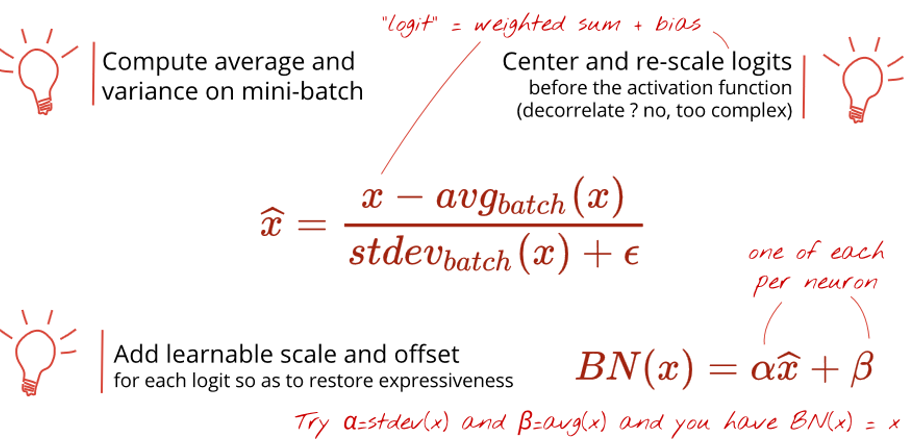
\includegraphics[width=\linewidth,keepaspectratio]{whitening}
\end{center}
\end{minipage}
}

\end{frame}


%%%%%%%%%%%%%%%%%%%%%%%%%%%%%%%%%%%%%%%%%%%%%%%%%%%
\begin{frame}[fragile] \frametitle{Batch Normalization in TensorFlow}
\begin{center}
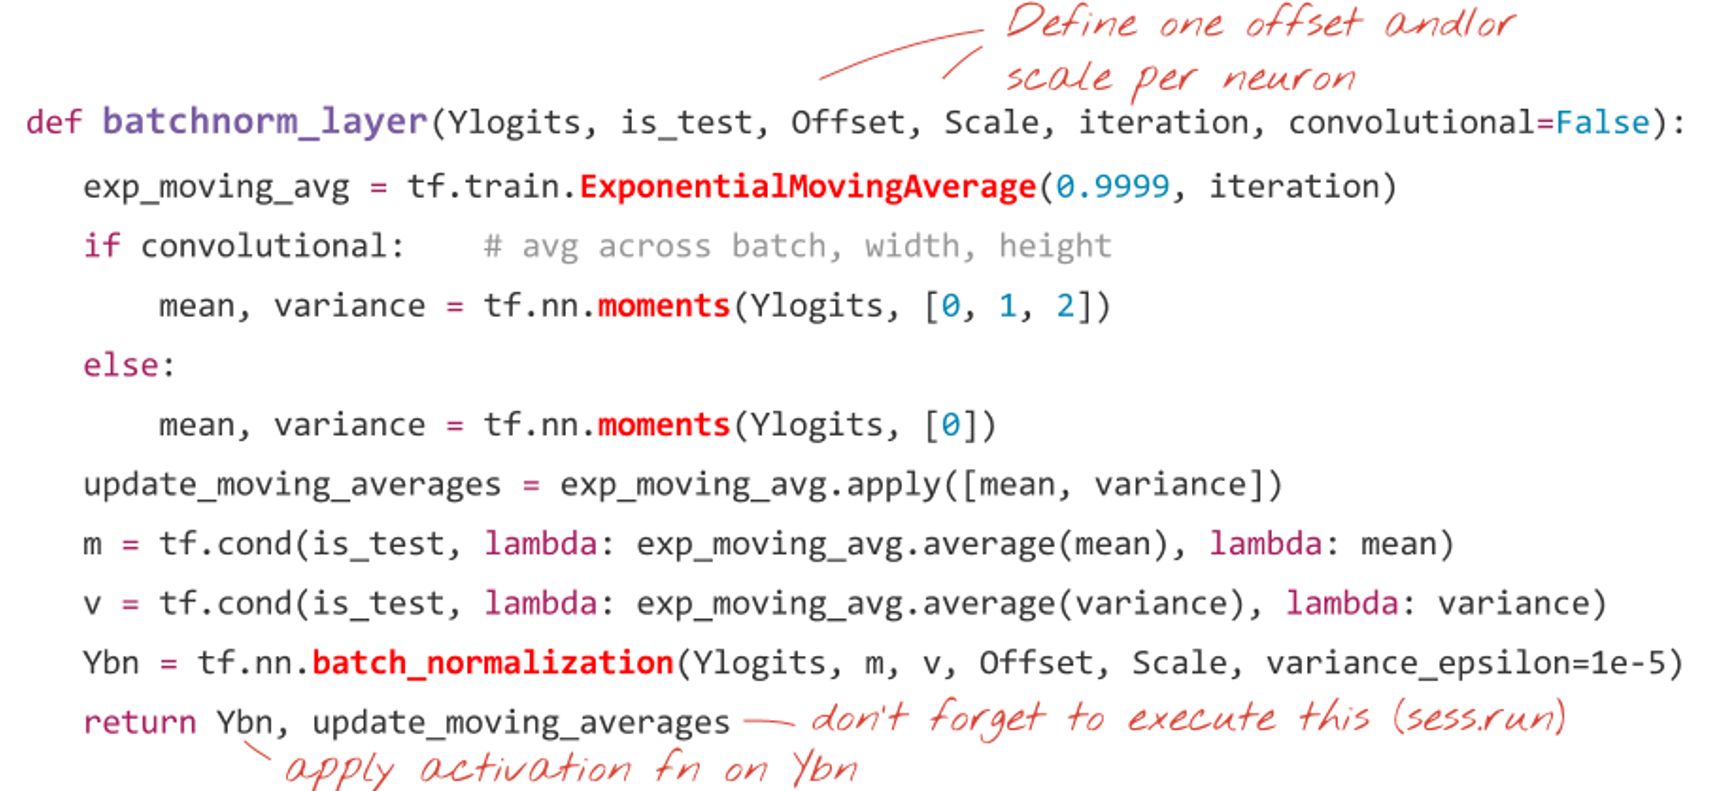
\includegraphics[width=\linewidth,keepaspectratio]{batchnorm}
\end{center}
\end{frame}


%%%%%%%%%%%%%%%%%%%%%%%%%%%%%%%%%%%%%%%%%%%%%%%%%%%
\begin{frame}
  \begin{center}
    {\Large Sample Example}
    
    (Ref: KD Nuggets, Ahmed Gad)
  \end{center}
\end{frame}

%%%%%%%%%%%%%%%%%%%%%%%%%%%%%%%%%%%%%%%%%%%%%%%%%%%
\begin{frame}[fragile] \frametitle{TensorFlow Steps}
\begin{itemize}
\item Reading the training data (inputs and outputs)
\item Building and connect the neural networks layers (this included preparing weights, biases, and activation function of each layer)
\item Building a loss function to assess the prediction error
\item Create a training loop for training the network and updating its parameters
\item Applying some testing data to assess the network prediction accuracy 
\end{itemize}
\end{frame}

%%%%%%%%%%%%%%%%%%%%%%%%%%%%%%%%%%%%%%%%%%%%%%%%%%%
\begin{frame}[fragile] \frametitle{Classification Problem}
\begin{center}
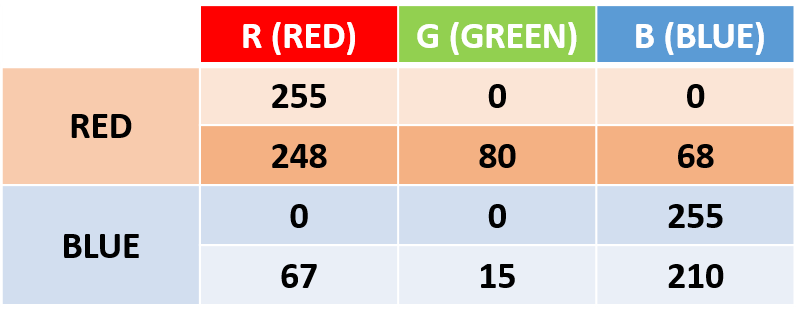
\includegraphics[width=0.6\linewidth,keepaspectratio]{kd1}
\end{center}
\begin{itemize}
\item It is a binary classification problem 
\item To classify colors into either red or blue
\item Based on the three RGB color channels.
\end{itemize}
\end{frame}

%%%%%%%%%%%%%%%%%%%%%%%%%%%%%%%%%%%%%%%%%%%%%%%%%%%
\begin{frame}[fragile] \frametitle{Classification Problem}

\begin{itemize}
\item It can be solved linearly and thus no need for hidden layers. 
\item Just input and output layers are to be used. 
\item There will be a single neuron in the output layer with an activation function.
\end{itemize}
\end{frame}


%%%%%%%%%%%%%%%%%%%%%%%%%%%%%%%%%%%%%%%%%%%%%%%%%%%
\begin{frame}[fragile] \frametitle{Classification Problem}

\begin{center}
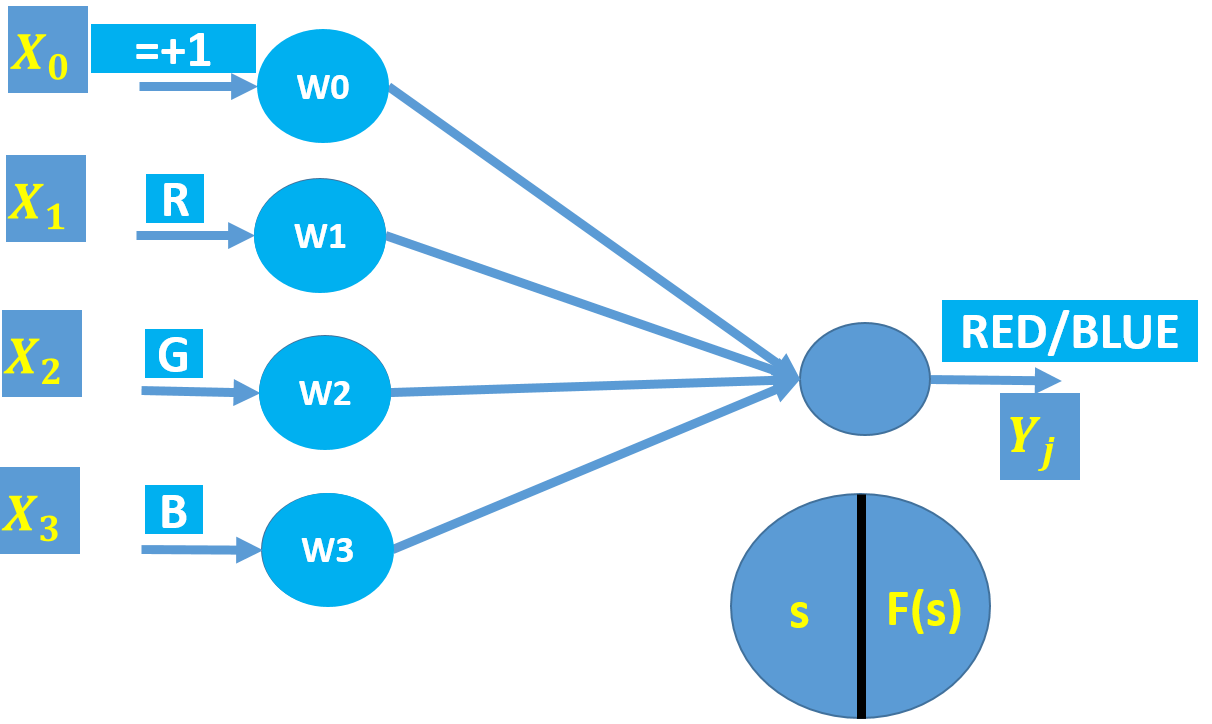
\includegraphics[width=0.6\linewidth,keepaspectratio]{kd2}
\end{center}
Where $X_0=1$ is the bias and W0 is its weight. W1 , W2, and W3 are the weights for the three inputs R (Red), G (Green), and B (Blue).
\end{frame}


%%%%%%%%%%%%%%%%%%%%%%%%%%%%%%%%%%%%%%%%%%%%%%%%%%%
\begin{frame}[fragile] \frametitle{Reading the Training Data}

\begin{itemize}
\item Data is read in placeholders.
\item Why we have not just used a NumPy array for preparing the data? 
\item To answer these questions, we can explore a simpler example that reads some inputs and print it to the console.
\end{itemize}
\end{frame}

%%%%%%%%%%%%%%%%%%%%%%%%%%%%%%%%%%%%%%%%%%%%%%%%%%%
\begin{frame}[fragile] \frametitle{Reading the Training Data}
\begin{lstlisting}
import tensorflow  
  
# Creating a NumPy array holding the input data  
numpy_inputs = [[5, 2, 13],  
    			             [7, 9, 0]]  
    			             
# Converting the NumPy array to a TensorFlow Tensor  
training_inputs = tensorflow.convert_to_tensor(value=numpy_inputs, dtype=tensorflow.int8)  

# Creating a TensorFlow Session  
sess = tensorflow.Session()  
  
# Running the session for evaluating the previously created Tensor  
print("Output is : ", sess.run(fetches=training_inputs))  
  
# Closing the TensorFlow Session  
sess.close()
\end{lstlisting}
\end{frame}


%%%%%%%%%%%%%%%%%%%%%%%%%%%%%%%%%%%%%%%%%%%%%%%%%%%
\begin{frame}[fragile] \frametitle{Reading the Training Data}

\begin{itemize}
\item The input is read into a NumPy array
\item Converted to Tensors as TensorFlow knows only about that.
\item \lstinline|Output is :  [[ 5  2 13] , [ 7  9  0]]|
\item This example doesn't use placeholders. 
\item So, what is the use of a TensorFlow placeholder? 
\end{itemize}
\end{frame}

%%%%%%%%%%%%%%%%%%%%%%%%%%%%%%%%%%%%%%%%%%%%%%%%%%%
\begin{frame}[fragile] \frametitle{Reading the Training Data}

\begin{itemize}
\item Assume that we want to run the session with another input. 
\item To do that, we have to modify the numpy\_input Python variable each time a new input is applied.
\item Placeholder in TensorFlow is a way for accepting the input data.
\item It is created in the code and modified multiple times in the Session running time. 
\end{itemize}
\end{frame}

%%%%%%%%%%%%%%%%%%%%%%%%%%%%%%%%%%%%%%%%%%%%%%%%%%%
\begin{frame}[fragile] \frametitle{Reading the Training Data}
\begin{lstlisting}
import tensorflow  
   
# Create a placeholder with data type int8 and shape 2x3.  
training_inputs = tensorflow.placeholder(dtype=tensorflow.int8, shape=(2, 3))  
   
# Creating a TensorFlow Session  
sess = tensorflow.Session()  
   
# Running the session for evaluating assigning a value to the placeholder  
print("Output is : ", sess.run(fetches=training_inputs,  
		feed_dict={training_inputs: [[5, 2, 13],  
                                                   [7, 9, 0]]}))  

# Closing the TensorFlow Session  
sess.close()  
\end{lstlisting}
This code prints the same outputs as before but it uses a placeholder.
\end{frame}

%%%%%%%%%%%%%%%%%%%%%%%%%%%%%%%%%%%%%%%%%%%%%%%%%%%
\begin{frame}[fragile] \frametitle{Reading the Training Data}

\begin{itemize}
\item The placeholder is created by specifying the data type and the shape of the data it will accept. 
\item The shape can be specified to restrict the input data to be of specific size.
\item If no shape specified, then different inputs with different shapes can be assigned to the placeholder.
\item The placeholder is assigned a value when running the Session using the feed\_dict argument of the run operation. 
\item  feed\_dict is a dictionary used to initialize the placeholders.
\end{itemize}
\end{frame}

%%%%%%%%%%%%%%%%%%%%%%%%%%%%%%%%%%%%%%%%%%%%%%%%%%%
\begin{frame}[fragile] \frametitle{Sampling the Training Data}

\begin{itemize}
\item But assume there is a feature vector of 50 feature and we have a dataset of 100 samples. 
\item Assume we want to train a model two times with different number of samples, say 30 and 40.
\item If you set it to 30 ie (30,50) you cant then change it to 40 (being fixed). 
\item So just leave it unspecified.
\end{itemize}
\begin{lstlisting}
# Create a placeholder with data type int8 and shape Rx3.  
training_inputs = tensorflow.placeholder(dtype=tensorflow.int8, shape=(None, 50))
\end{lstlisting}
\end{frame}


%%%%%%%%%%%%%%%%%%%%%%%%%%%%%%%%%%%%%%%%%%%%%%%%%%%
\begin{frame}[fragile] \frametitle{Sampling the Training Data}

\begin{itemize}
\item Benefit of placeholder is that its value is modified easily. 
\item You have not to modify the program for different inputs. 
\item We can run the session multiple times with different values for the placeholder:
\end{itemize}
\begin{lstlisting}
# Running the session for evaluating assigning a value to the placeholder  
print("Output is : ", sess.run(fetches=training_inputs,  feed_dict={training_inputs: [[5, 2, 13],  [7, 9, 0]]}))  
print("Output is : ", sess.run(fetches=training_inputs, feed_dict={training_inputs: [[1, 2, 3],  [4, 5, 6]]}))  
print("Output is : ", sess.run(fetches=training_inputs,  feed_dict={training_inputs: [[12, 13, 14],  [15, 16, 17]]}))
\end{lstlisting}
\end{frame}

%%%%%%%%%%%%%%%%%%%%%%%%%%%%%%%%%%%%%%%%%%%%%%%%%%%
\begin{frame}[fragile] \frametitle{Sampling the Training Data}

\begin{itemize}
\item To do that using NumPy arrays we have to create a new Python array for each new input.
\item This is why we are using placeholders for feeding the data. 
\item For every input there should be a separate placeholder.
\item In out neural network, there are two inputs which are training inputs and training outputs and thus there should be two placeholders one for each
\end{itemize}
\begin{lstlisting}
# Preparing training data (inputs-outputs)  
training_inputs = tensorflow.placeholder(shape=[None, 3], dtype=tensorflow.float32)  
training_outputs = tensorflow.placeholder(shape=[None, 1], dtype=tensorflow.float32) #Desired outputs for each input 
\end{lstlisting}

\end{frame}

%%%%%%%%%%%%%%%%%%%%%%%%%%%%%%%%%%%%%%%%%%%%%%%%%%%
\begin{frame}[fragile] \frametitle{Sampling the Training Data}

\begin{itemize}
\item Note that the size of these placeholders is not fixed to allow variable number of training samples to be used with the code unchanged. 
\item But both placeholders of inputs and outputs training data must have the same number of rows. 
\item For example, according to our currently presented training data, training\_inputs should have a shape=(4, 2) and training\_outputs should be of shape=(4, 1).
\end{itemize}

\end{frame}

%%%%%%%%%%%%%%%%%%%%%%%%%%%%%%%%%%%%%%%%%%%%%%%%%%%
\begin{frame}[fragile] \frametitle{Preparing the Neural Network }

\begin{itemize}
\item What type to choose for Weights.
\item Placeholders can not be chosen.
\item Placeholder value can't be changed once assigned. 
\item After it is given a value then placeholder can be regarded a constant. 
\item Thus it is not the suitable option for trainable parameters
\item Trainable parameter is assigned an initial value and that value got changed until reaching the best value making the underlying model produce least errors.
\end{itemize}

\end{frame}

%%%%%%%%%%%%%%%%%%%%%%%%%%%%%%%%%%%%%%%%%%%%%%%%%%%
\begin{frame}[fragile] \frametitle{Preparing the Neural Network }

\begin{itemize}
\item For our neural network, there are two trainable parameters which are weight and bias.
\item These parameters are not suitable for being stored in placeholders as we want to update them until getting their best values. 
\item This is why there is something in TensorFlow called Variable.
\end{itemize}

\end{frame}

%%%%%%%%%%%%%%%%%%%%%%%%%%%%%%%%%%%%%%%%%%%%%%%%%%%
\begin{frame}[fragile] \frametitle{Preparing the Neural Network }

To create a TensorFlow Variable, specify type and shape.
\begin{lstlisting}
import tensorflow  

# Create a Variable with data type int8 and shape 2x3. 
training_inputs = tensorflow.Variable(initial_value=[[5, 2, 13],  [7, 9, 0]], dtype=tensorflow.int8)

sess = tensorflow.Session() 

# Initialize all Variables  
sess.run(tensorflow.global_variables_initializer())  

# Running the session for evaluating assigning a value to the placeholder  
print("Output is : ", sess.run(fetches=training_inputs))  
sess.close() 
\end{lstlisting}
Note that the Variable won't be initialized until calling the global\_variables\_initializer() 
\end{frame}

%%%%%%%%%%%%%%%%%%%%%%%%%%%%%%%%%%%%%%%%%%%%%%%%%%%
\begin{frame}[fragile] \frametitle{Preparing the Neural Network }

There are two variables created for our two parameters: weight and bias
\begin{lstlisting}
# Preparing neural network parameters (weights and bias) using TensorFlow Variables  
weights = tensorflow.Variable(initial_value=[[.3], [.1], [.8]], dtype=tensorflow.float32)  
bias = tensorflow.Variable(initial_value=[[1]], dtype=tensorflow.float32)  
\end{lstlisting}
Note that they both weight and bias has initial values. 
\end{frame}

%%%%%%%%%%%%%%%%%%%%%%%%%%%%%%%%%%%%%%%%%%%%%%%%%%%
\begin{frame}[fragile] \frametitle{Preparing the Neural Network }

\begin{itemize}
\item We are using fixed initial values for them. The initial values are set randomly and there is no rule used for generating them.
\item You may use any random number generation operation in TensorFlow for doing that such as tensorflow.truncated\_normal().
\item But note that the initial values are critical for creating a robust model able to predict the right class after being trained. 
\item Bad initial values for weights and bias of a neural network can make its neurons to die. 
\item This is why there are many techniques used to generate such initial values.
\end{itemize}

\end{frame}

%%%%%%%%%%%%%%%%%%%%%%%%%%%%%%%%%%%%%%%%%%%%%%%%%%%
\begin{frame}[fragile] \frametitle{Preparing the Neural Network }
As a summary:
\begin{itemize}
\item A placeholder is used to store input data that are to be initialized once and used multiple times.
\item But Variable is used for trainable parameters that are to be changed multiple times after being initialized.
\end{itemize}

\end{frame}

%%%%%%%%%%%%%%%%%%%%%%%%%%%%%%%%%%%%%%%%%%%%%%%%%%%
\begin{frame}[fragile] \frametitle{Preparing the Neural Network }
Our activation function is used to merge all inputs, weights, and bias into a single value describing the expected class score of each input.
\begin{lstlisting}
# Activation function of the output layer neuron  
predictions = tensorflow.nn.sigmoid(af_input)  
\end{lstlisting}
\end{frame}

%%%%%%%%%%%%%%%%%%%%%%%%%%%%%%%%%%%%%%%%%%%%%%%%%%%
\begin{frame}[fragile] \frametitle{Matrix Multiplication}

\begin{itemize}
\item Normally, there is a weight for each input. Each input is multiplied by its corresponding weight. 
\item We don't have to make element-by-element multiplications and matrix multiplication can be a good solution.
\item Just prepare a matrix for inputs and another one for weights and multiply these two matrices. 
\item The tensorflow.matmul() operation make that for you.
\end{itemize}
\begin{lstlisting}
# Preparing inputs of the activation function  
af_input = tensorflow.matmul(training_inputs, weights) + bias  
\end{lstlisting}
\end{frame}

%%%%%%%%%%%%%%%%%%%%%%%%%%%%%%%%%%%%%%%%%%%%%%%%%%%
\begin{frame}[fragile] \frametitle{Prediction Error}

\begin{itemize}
\item Evaluating the model is an essential step after it has been trained. 
\item This is why there is a loss function.
\item Just find the difference between each desired output and its corresponding predicted output by the model. 
\item To find a single value representing the overall error of the network, the summation of individual differences is calculated using the tensorflow.reduce\_sum() operation.
\end{itemize}
\begin{lstlisting}
# Measuring the prediction error of the network after being trained  
prediction_error = tensorflow.reduce_sum(training_outputs - predictions)
\end{lstlisting}
\end{frame}

%%%%%%%%%%%%%%%%%%%%%%%%%%%%%%%%%%%%%%%%%%%%%%%%%%%
\begin{frame}[fragile] \frametitle{Updating Network Parameters}

\begin{itemize}
\item The prediction error of the model may not be zero from the first trial and it may be very high. 
\item This is why there must be a way for automatically updating and optimizing the model parameters to get the least possible error.
\item One of the common optimizers is gradient descent (GD). GD tries to find the relationship between each parameter and the prediction error to know how each parameter affects the error.
\end{itemize}
\end{frame}


%%%%%%%%%%%%%%%%%%%%%%%%%%%%%%%%%%%%%%%%%%%%%%%%%%%
\begin{frame}[fragile] \frametitle{Updating Network Parameters}

\begin{itemize}
\item First trying the initial parameters. If they didn`t do well, then GD will try to change the parameters values and moving toward the direction that minimizes the error. 
\item The GD optimizer is applied in our example to minimize the previously calculated prediction error. 
\item The learning\_rate of the tensorflow.train.GradientDescentOptimizer is just a hyper-parameter.
\end{itemize}
\begin{lstlisting}
# Minimizing the prediction error using gradient descent optimizer  
train_op = tensorflow.train.GradientDescentOptimizer(learning_rate=0.05).minimize(prediction_error) 
\end{lstlisting}
\end{frame}


%%%%%%%%%%%%%%%%%%%%%%%%%%%%%%%%%%%%%%%%%%%%%%%%%%%
\begin{frame}[fragile] \frametitle{Training Loop}
\begin{itemize}
\item The remaining step is to go into a loop that updates the parameters automatically.
\item After that we can run the training loop .
\item Note that the only parameter specified to be fetched is the Tensor returned by tensorflow.train.GradientDescentOptimizer which is train\_op.
\item  This is because fetching train\_op will cause all parameters to be updated. 
\end{itemize}
\end{frame}

%%%%%%%%%%%%%%%%%%%%%%%%%%%%%%%%%%%%%%%%%%%%%%%%%%%
\begin{frame}[fragile] \frametitle{Training Loop}
The loop will last for 10,000 iterations and at each iteration the GD optimizer will generate new values for the parameters that decreases the error.
\begin{lstlisting}
# Training loop of the neural network  
for step in range(10000):  
    sess.run(fetches=[train_op], feed_dict={
                                 training_inputs: training_inputs_data,  
                                 training_outputs: training_outputs_data}) 
\end{lstlisting}
\end{frame}

%%%%%%%%%%%%%%%%%%%%%%%%%%%%%%%%%%%%%%%%%%%%%%%%%%%
\begin{frame}[fragile] \frametitle{Updating Network Parameters}

\begin{itemize}
\item Because data are stored into placeholders, then these placeholders must be initialized using the feed\_dict argument of the tensorflow.Session.run() operation. 
\item The weights and bias placeholders are initialized using a previously created NumPy arrays 
\item We can also avoid creating a separate NumPy arrays and make assign the data to the placeholders within the run() operation as follows:
\end{itemize}
\begin{lstlisting}
# Training loop of the neural network  
for step in range(10000):  
    sess.run(fetches=[train_op], feed_dict={training_inputs: [[255, 0, 0],  [248, 80, 68],  [0, 0, 255],  [67, 15, 210]]  ,  
                    training_outputs: [[1],  [1],  [0],  [0]]})
\end{lstlisting}
But for code clarity, the NumPy arrays are created separately from the run() operation.
\end{frame}

%%%%%%%%%%%%%%%%%%%%%%%%%%%%%%%%%%%%%%%%%%%%%%%%%%%
\begin{frame}[fragile] \frametitle{Testing the Trained Neural Network}

\begin{itemize}
\item After getting out of the training loop, the neural network will be trained and ready for predicting unknown samples. 
\item Two new samples were used for testing the network accuracy.
\end{itemize}
\begin{lstlisting}
# Predicted classes of some testing data  
print("Expected Class Scores : ", sess.run(fetches=predictions, 
feed_dict={training_inputs: [[255, 100, 50],   [100,50,255]]   
\end{lstlisting}
The expected class scores are as follows:
\begin{lstlisting}
Expected class scores :  [[ 1.]  [ 1.]]   
\end{lstlisting}
\end{frame}


%%%%%%%%%%%%%%%%%%%%%%%%%%%%%%%%%%%%%%%%%%%%%%%%%%%
\begin{frame}[fragile] \frametitle{Testing the Trained Neural Network}

\begin{itemize}
\item This is not accurate result because it say that the expected class score of the two samples is indexed 1 which is the BLUE class. 
\item The reason is the bad use of the initial values for the network parameters (weights and bias). 
\item We can try using different initial values and see how the results get changed. 
\item For example, using the tensorflow.truncated\_normal() operation, we can generate the initial values for both weights and bias as follows:
\end{itemize}
\begin{lstlisting}
# Preparing neural network parameters (weights and bias) using TensorFlow Variables  
weights = tensorflow.Variable(tensorflow.truncated_normal(shape=[3, 1], dtype=tensorflow.float32))  
bias = tensorflow.Variable(tensorflow.truncated_normal(shape=[1, 1], dtype=tensorflow.float32)) 
\end{lstlisting}
\end{frame}

%%%%%%%%%%%%%%%%%%%%%%%%%%%%%%%%%%%%%%%%%%%%%%%%%%%
\begin{frame}[fragile] \frametitle{Testing the Trained Neural Network}

\begin{itemize}
\item Then we can train the network again using the newly used initial values and predict the results again. 
\item The result of expectation is as follows:
\end{itemize}
\begin{lstlisting}
Expected class score :  [[  3.23404099e-23]  [  1.00000000e+00]]
\end{lstlisting}
The new values for the weights and bias can be printed as follows:
\begin{lstlisting}
print("Weights : ", sess.run(weights))  
print("Bias : ", sess.run(bias)) 
Weights :  [[-0.20039153]  [-0.91293597]  [ 0.44236434]]  
 Bias :  [[-0.685884]]  
\end{lstlisting}
\end{frame}

%%%%%%%%%%%%%%%%%%%%%%%%%%%%%%%%%%%%%%%%%%%%%%%%%%%
\begin{frame}[fragile] \frametitle{Testing the Trained Neural Network}

\begin{itemize}
\item The results enhanced so much and the error is now 0.0 compared to 1.0 in the previous fixed initial values. 
\item This proves the importance of initializing the neural networks weights well.
\end{itemize}

\end{frame}












%%%%%%%%%%%%%%%%%%%%%%%%%%%%%%%%%%%%%%%%%%%%%%%%%%%
\begin{frame}
  \begin{center}
    {\Large Sample Example}
    
    MNIST: Image Classification
  \end{center}
\end{frame}


%%%%%%%%%%%%%%%%%%%%%%%%%%%%%%%%%%%%%%%%%%%%%%%%%%%
\begin{frame}[fragile] \frametitle{MNIST: recognize Hand written digits}
\begin{center}
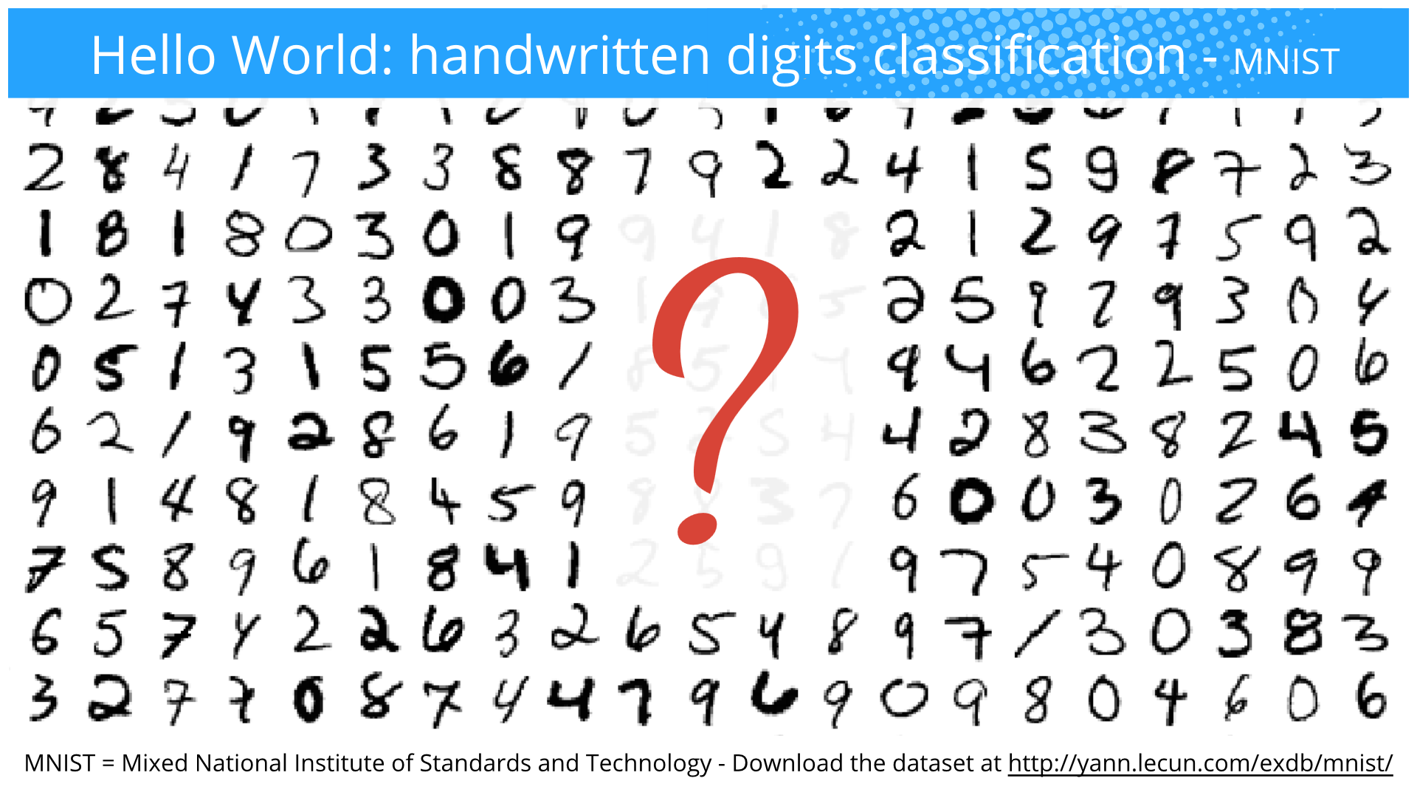
\includegraphics[width=0.8\linewidth,keepaspectratio]{mnistclass}
\end{center}
\end{frame}

%%%%%%%%%%%%%%%%%%%%%%%%%%%%%%%%%%%%%%%%%%%%%%%%%%%
\begin{frame}[fragile] \frametitle{Data Set}

\begin{itemize}
\item mnist.train has 55k data points, mnist.test has 10k and mnist.validation has 5k mnist.train.images are the x and mnist.train.labels are y
\item Each image is 28x28 pixel so 784 numbers in a flattened array
\item Model to be used is SOFTMAX regression because it gives us a list of values between 0 and 1 that add up to 1. Two steps: 
\begin{itemize}
\item we add up the evidence of our input being in certain classes, 
\item we convert that evidence into probabilities
\end{itemize}
\end{itemize}

\end{frame}

%%%%%%%%%%%%%%%%%%%%%%%%%%%%%%%%%%%%%%%%%%%%%%%%%%%
\begin{frame}[fragile] \frametitle{Simple Neural Network}

\begin{itemize}
\item 28x28 pixel image is flattened into a single row of 784 pixel intensities
\item These act as $x_1,x_2$ input nodes. 
\item Softmax layer is of dim 784 (input dim) x 10 (output dim) who calculates probabilities from 0 to 1, with $8$ having the maximum probability.
\end{itemize}
\begin{center}
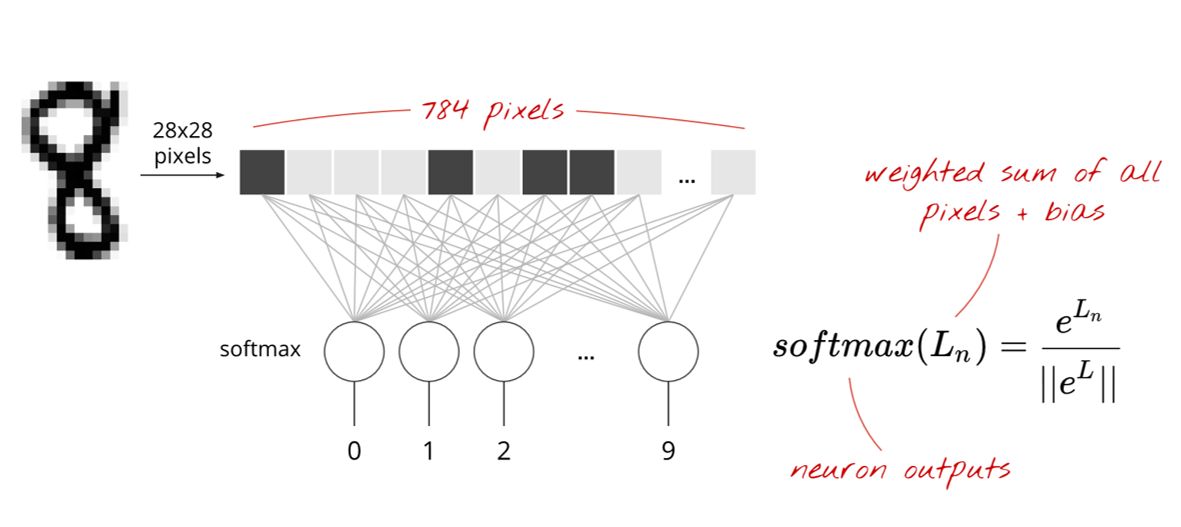
\includegraphics[width=0.8\linewidth,keepaspectratio]{mnistnn}
\end{center}
\end{frame}

%%%%%%%%%%%%%%%%%%%%%%%%%%%%%%%%%%%%%%%%%%%%%%%%%%%
\begin{frame}[fragile] \frametitle{Input with 100 images at a time}

\begin{itemize}
\item $X (100x784)*W(784x10) + b(10)$
\item Bias added `broadcasted'
\item Copied smaller row to all 
\end{itemize}
\begin{center}
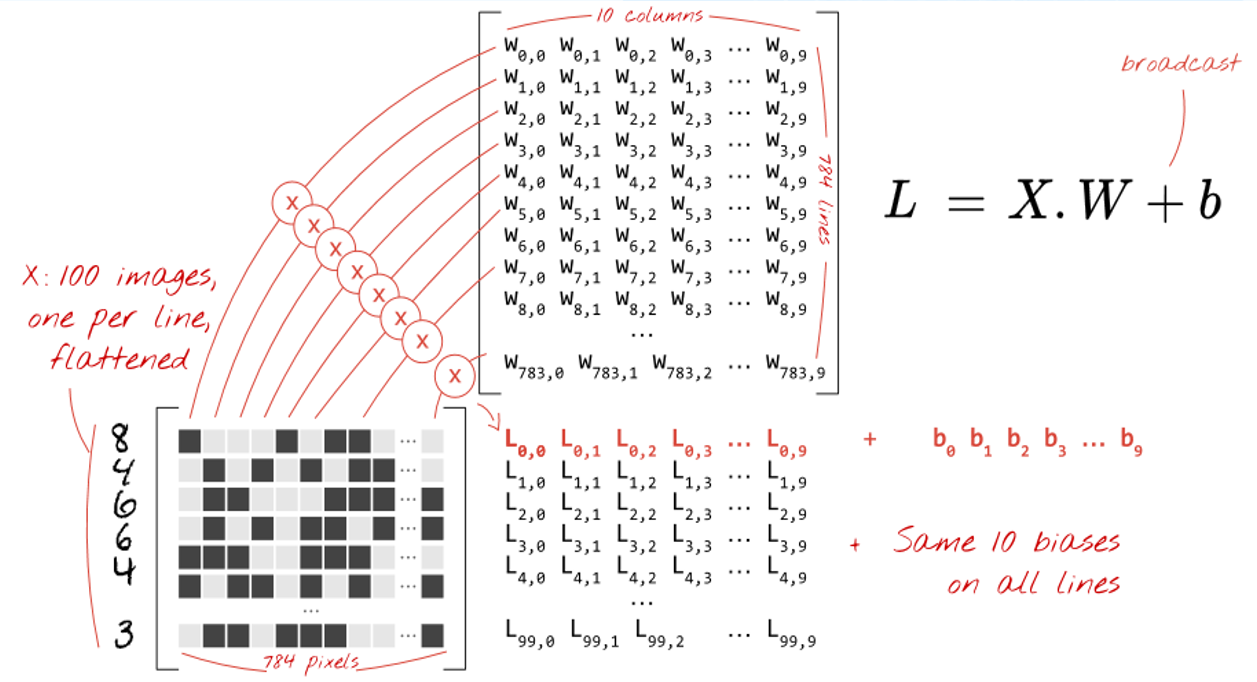
\includegraphics[width=0.8\linewidth,keepaspectratio]{mnistmat}
\end{center}
\end{frame}

%%%%%%%%%%%%%%%%%%%%%%%%%%%%%%%%%%%%%%%%%%%%%%%%%%%
\begin{frame}[fragile] \frametitle{Finally, softmax}

\begin{itemize}
\item Softmax takes weighted sum + bias, line by line. Elevates each to e
\item Then normalizes with addition from all (L1: addition; L2: sqr addition)
\item Output is y,ie 100 images with 10 values of probabilities for each digit
\item Max probability is the result
\end{itemize}
\begin{center}
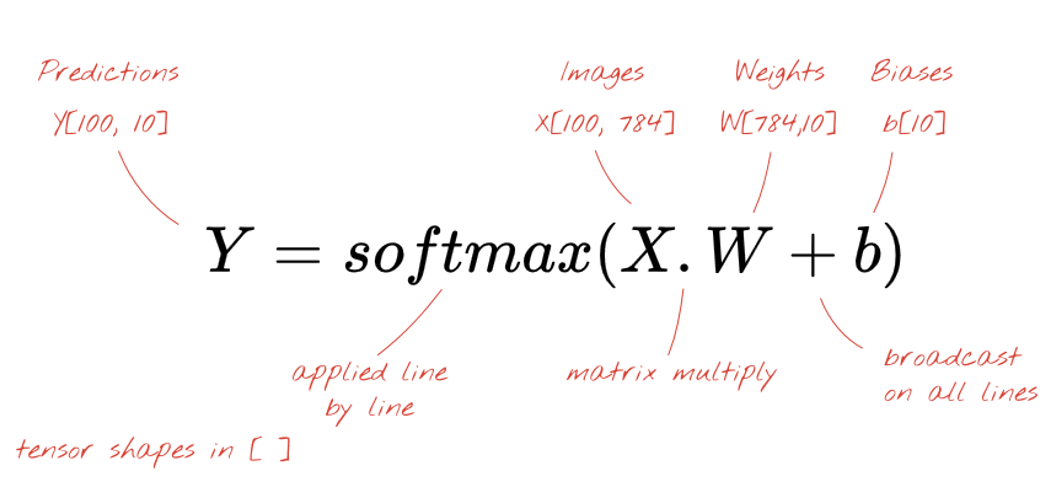
\includegraphics[width=0.8\linewidth,keepaspectratio]{mnistsoftmax}
\end{center}
\end{frame}

%%%%%%%%%%%%%%%%%%%%%%%%%%%%%%%%%%%%%%%%%%%%%%%%%%%
\begin{frame}[fragile] \frametitle{Train: Define loss and minimize it}

\begin{itemize}
\item Error(Loss) is diff between Actual and predicted probabilities
\item Cross Entropy one of the ways to define this error.
\item Its dot product, element wise product of y and log of predicted.
\item As y-preds are < 1, logs are -ve
\item Overall -ve makes value +ve
\end{itemize}
\begin{center}
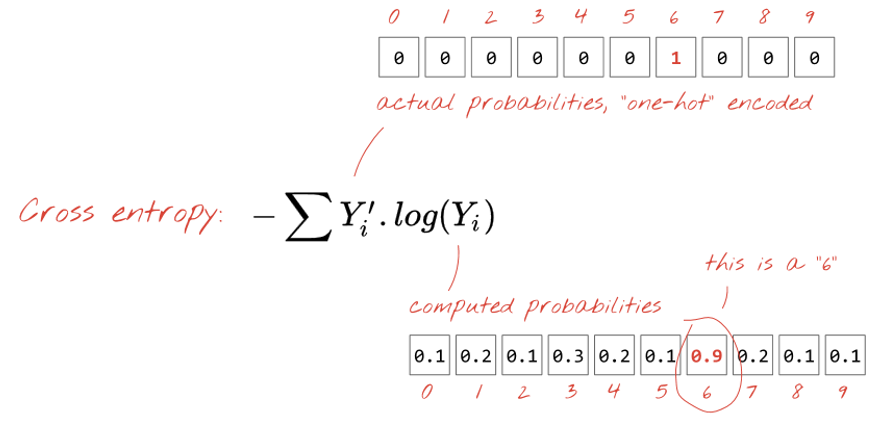
\includegraphics[width=0.8\linewidth,keepaspectratio]{mnistcross}
\end{center}
\end{frame}


%%%%%%%%%%%%%%%%%%%%%%%%%%%%%%%%%%%%%%%%%%%%%%%%%%%
\begin{frame}[fragile] \frametitle{TensorFlow implementation}

\begin{itemize}
\item $1$ number of values. For just intensities of grey scale, being just one value its 1. If color, then 3 values for RGB.
\item reshape flattens the matrix
\item $-1$ there, acts as $None$.
\end{itemize}
\begin{center}
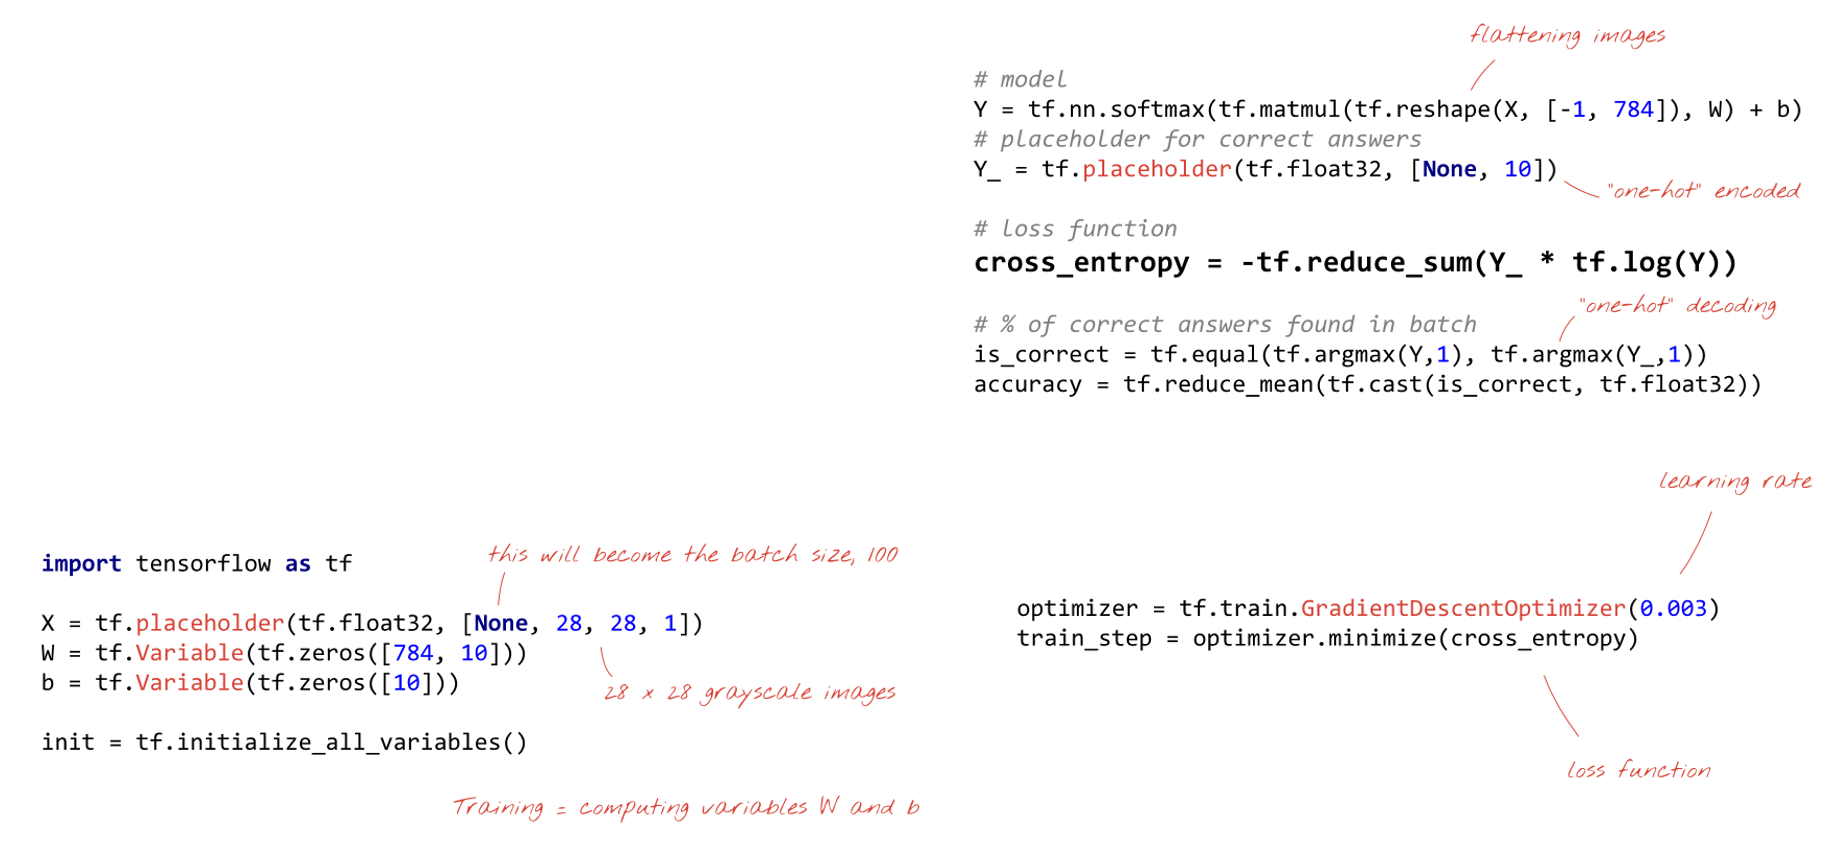
\includegraphics[width=\linewidth,keepaspectratio]{mnisttf}
\end{center}
\end{frame}

%%%%%%%%%%%%%%%%%%%%%%%%%%%%%%%%%%%%%%%%%%%%%%%%%%%
\begin{frame}[fragile] \frametitle{Full Python code}
\begin{center}
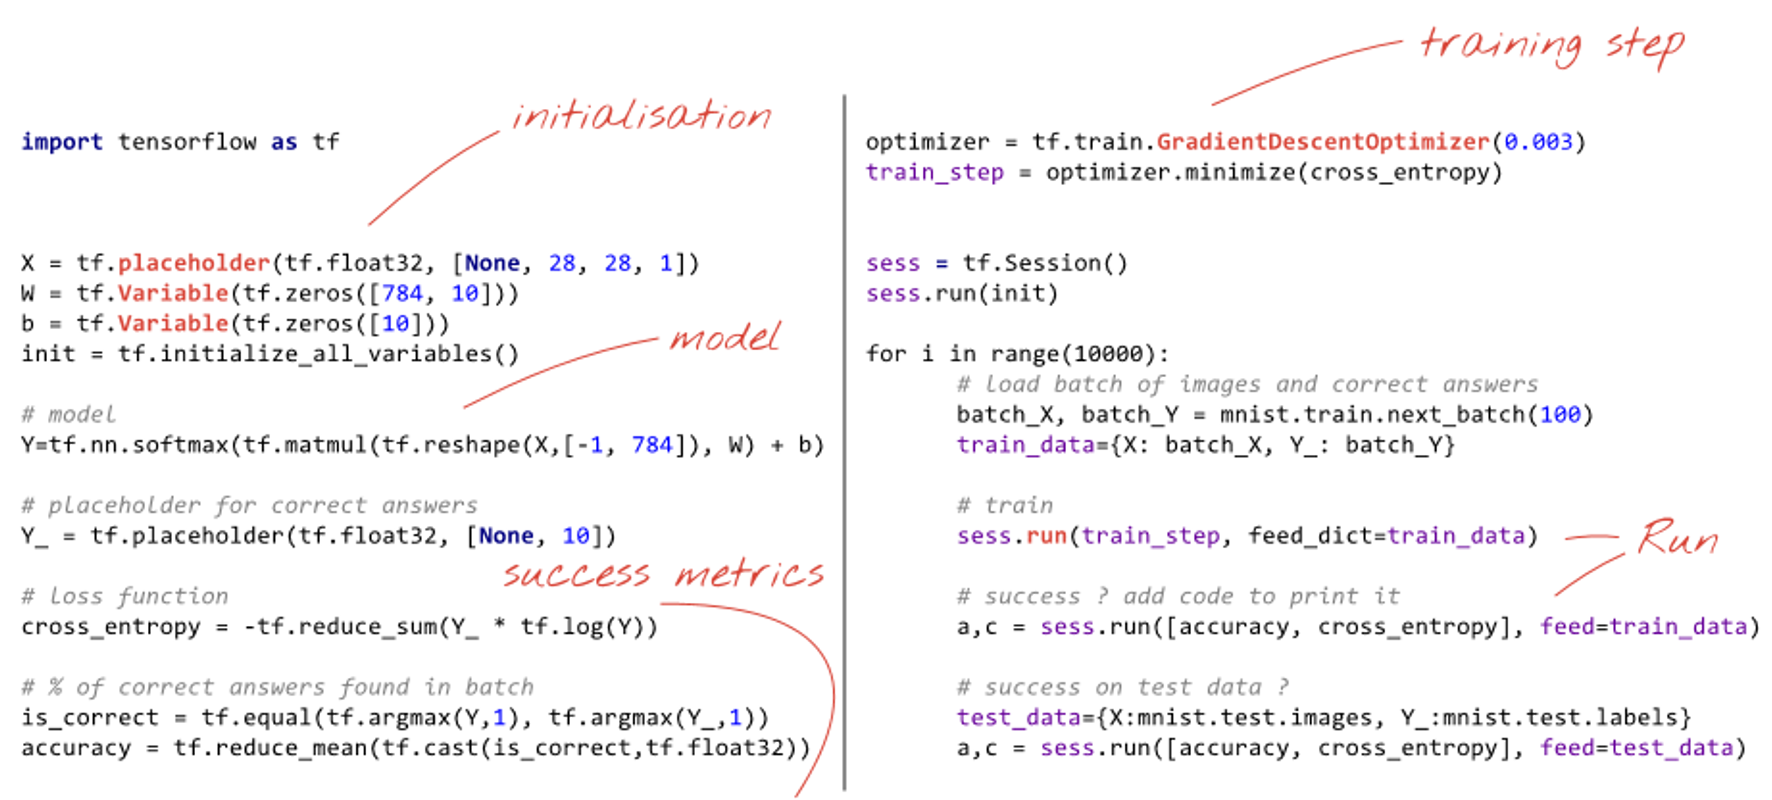
\includegraphics[width=\linewidth,keepaspectratio]{tfpy}
\end{center}
\end{frame}

%%%%%%%%%%%%%%%%%%%%%%%%%%%%%%%%%%%%%%%%%%%%%%%%%%%
\begin{frame}[fragile] \frametitle{What next?}

\begin{itemize}
\item 92\% accuracy not good enough. How to increase it?
\item Add more layers, with diff activation - sigmoid (0 to1, continuous)
\end{itemize}
\begin{center}
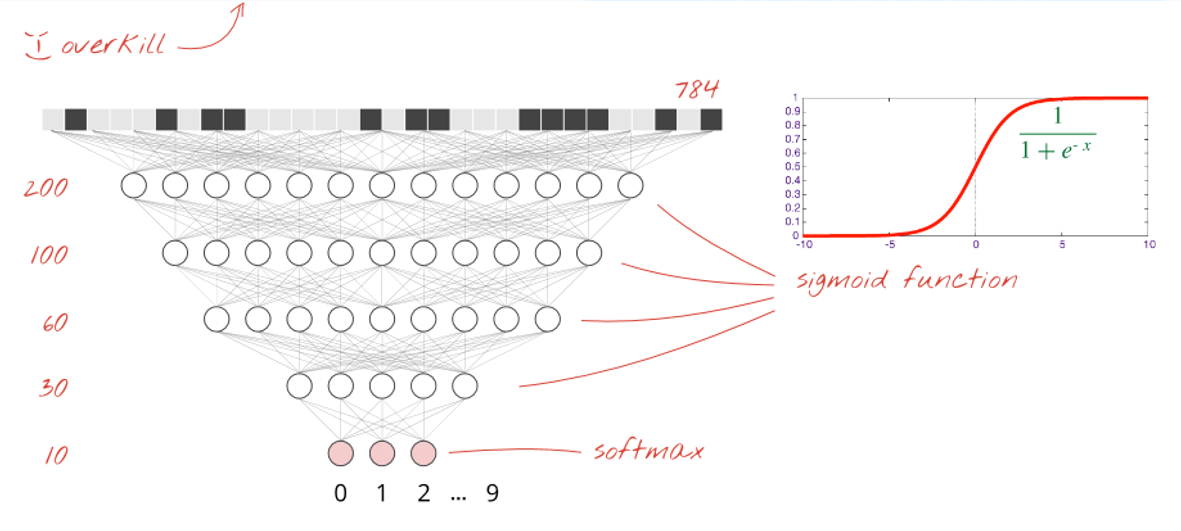
\includegraphics[width=\linewidth,keepaspectratio]{mnistsigmoid}
\end{center}
\end{frame}


%%%%%%%%%%%%%%%%%%%%%%%%%%%%%%%%%%%%%%%%%%%%%%%%%%%
\begin{frame}[fragile] \frametitle{Passing values between layers}
\begin{center}
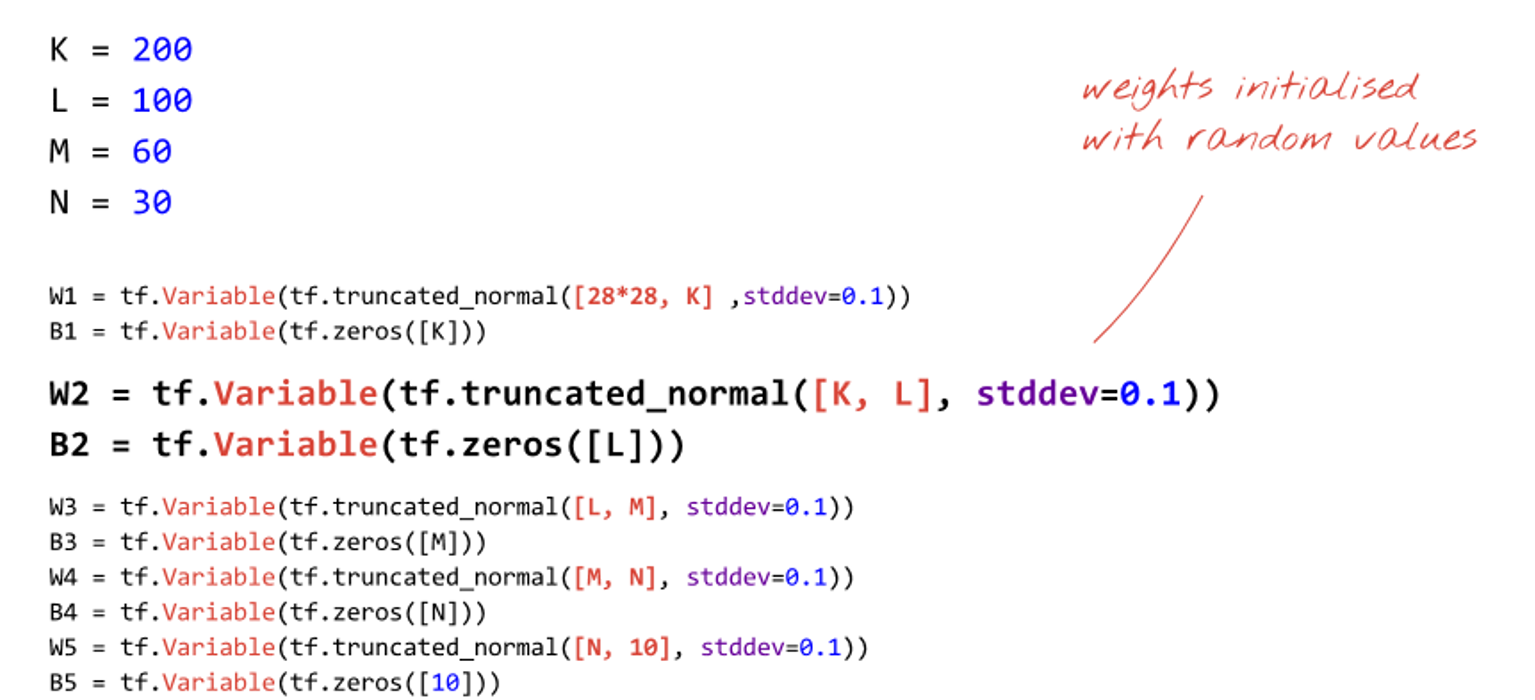
\includegraphics[width=\linewidth,keepaspectratio]{mnistpass}
\end{center}
\end{frame}


%%%%%%%%%%%%%%%%%%%%%%%%%%%%%%%%%%%%%%%%%%%%%%%%%%%
\begin{frame}[fragile] \frametitle{The model}
\begin{center}
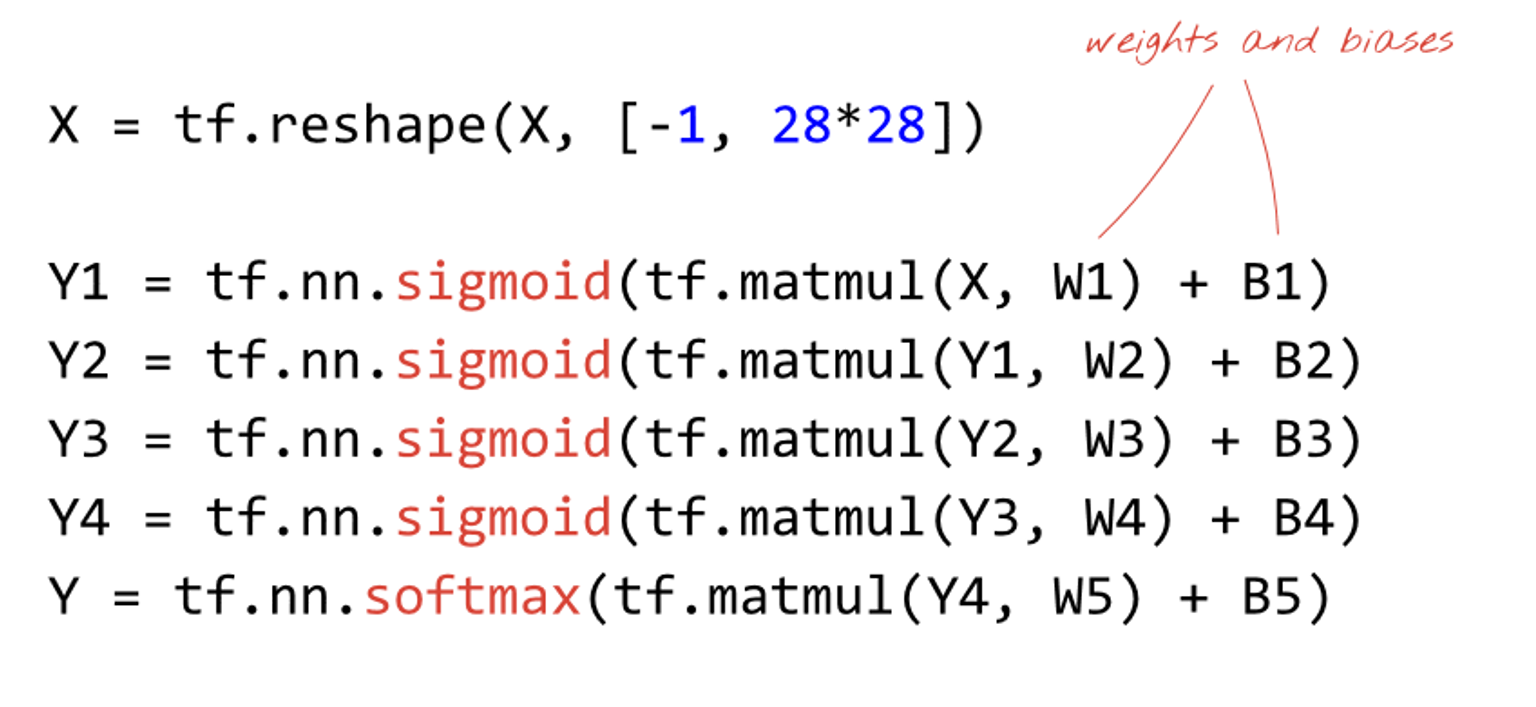
\includegraphics[width=\linewidth,keepaspectratio]{tfmodel}
\end{center}
Accuracy does not grow nicely, so instead of sigmoid, use RELU
\end{frame}

%%%%%%%%%%%%%%%%%%%%%%%%%%%%%%%%%%%%%%%%%%%%%%%%%%%
\begin{frame}[fragile] \frametitle{RELU}
\begin{center}
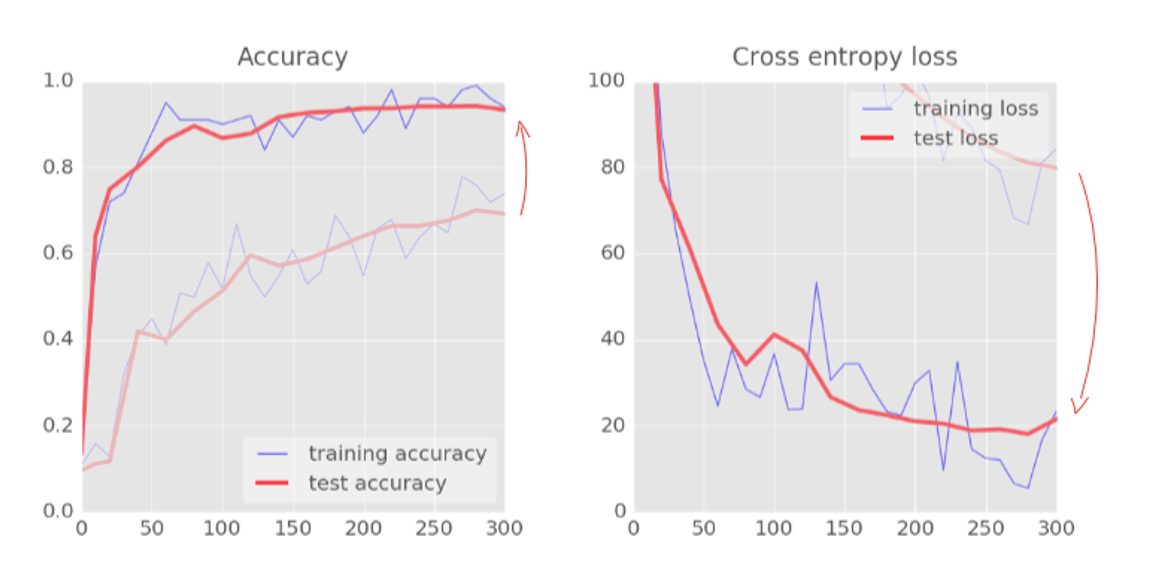
\includegraphics[width=\linewidth,keepaspectratio]{reluacc}
\end{center}
Accuracy shoots up sharply to 98\%
\end{frame}

%%%%%%%%%%%%%%%%%%%%%%%%%%%%%%%%%%%%%%%%%%%%%%%%%%%
\begin{frame}[fragile] \frametitle{Noisy accuracy graph (red)}

\begin{itemize} 
\item Learning rate is too fast. Reducing it would take lot of time.
\item What's needed is rate dropping sharply first, then decaying slowly
\item Cross entropy going up is Over fitting
\end{itemize}
\begin{center}
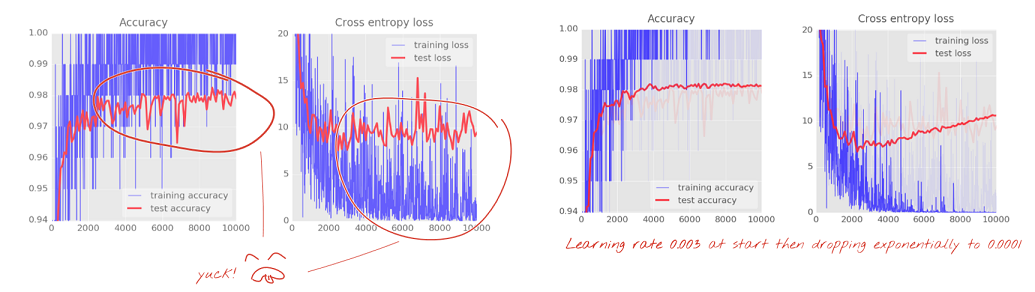
\includegraphics[width=\linewidth,keepaspectratio]{mnistacc}
\end{center}
\end{frame}


%%%%%%%%%%%%%%%%%%%%%%%%%%%%%%%%%%%%%%%%%%%%%%%%%%%
\begin{frame}[fragile] \frametitle{Regularization : Dropout}

\begin{itemize}
\item At each training iteration, shoot, say 25\% neurons, randomly. 
\item For next iteration, put them back, shoot another 25\% randomly
\item For testing, put all back.
\item Shoot means, W=0
\item To keep balance,
\item Increase, other weights proportionately
\end{itemize}
\begin{center}
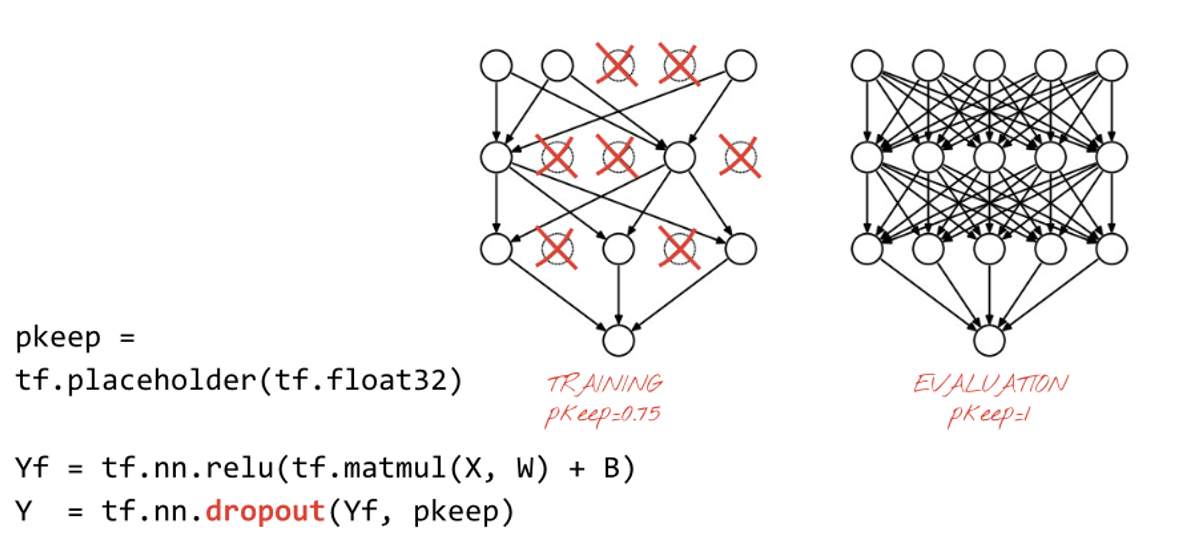
\includegraphics[width=0.6\linewidth,keepaspectratio]{mnistdrop}
\end{center}
\end{frame}

%%%%%%%%%%%%%%%%%%%%%%%%%%%%%%%%%%%%%%%%%%%%%%%%%%%
\begin{frame}[fragile] \frametitle{Experiments done so far}

\begin{itemize}
\item Simple Neural network (no hidden layer): 92\%
\item 5 layers with sigmoid at hidden layers, rate 0.003: 97.5\%
\item 5 layers, RELU at hidden, rate 0.003 : 98.2\%
\item 5 layers, RELU at hidden, decaying rate 0.003 to 0.0001: 98.2\% (smoother)
\item Above + dropout 0.75: 98.2\% but removes the overfitting in cross entropy
\end{itemize}
\begin{center}
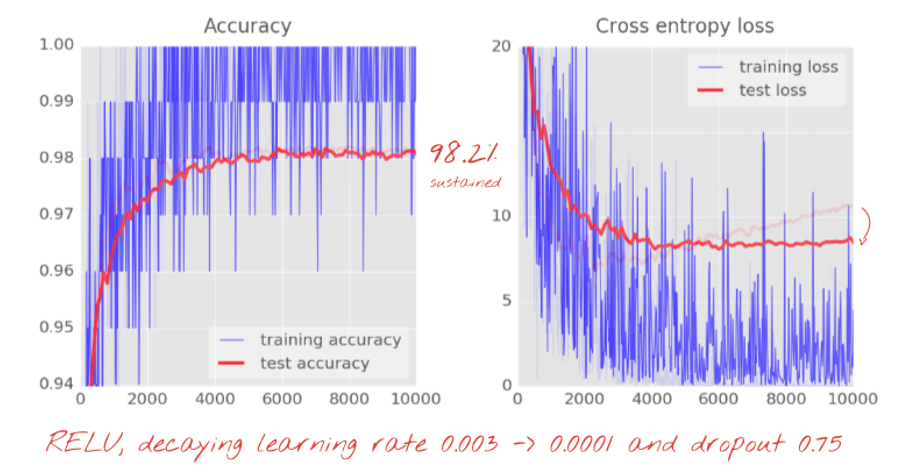
\includegraphics[width=0.6\linewidth,keepaspectratio]{mnistrelu}
\end{center}
\end{frame}

%%%%%%%%%%%%%%%%%%%%%%%%%%%%%%%%%%%%%%%%%%%%%%%%%%%
\begin{frame}[fragile] \frametitle{What is over-fitting, why drop out helps?}
\begin{itemize}
\item Too many weights, so too many degrees of freedom for training data
\item Why not reduce neurons or weights, so as to generalize better.
\item Can we do better? 
\item Reducing number of layers, does not help.
\item The current network architecture itself is inadequate!!!
\item Because we FLATTENED images. The local shape information is LOST.
\item Use Convolution, for where local shapes are important.
\end{itemize}
\end{frame}